\chapter{Études de cas}

\input{examples/Knuth_FR}

% sections here
\mysection{Fonction presque vide}
\label{Boolector}
\myindex{Boolector}
\myindex{x86!\Instructions!JMP}

Ceci est un morceau de code réel que j'ai trouvé dans Boolector\footnote{\url{https://boolector.github.io/}}:

\lstinputlisting[style=customc]{patterns/025_almost_empty/boolectormain.c}

Pourquoi quelqu'un ferait-il comme ça?
Je ne sais pas mais mon hypothèse est que \verb|boolector_main()| peut être compilée
dans une sorte de DLL ou bibliothèque dynamique, et appelée depuis une suite de test.
Certainement qu'une suite de test peut préparer les variables argc/argv comme
le ferait \ac{CRT}.

Il est intéressant de voir comment c'est compilé:

\lstinputlisting[caption=GCC 8.2 x64 \NonOptimizing (\assemblyOutput),style=customasmx86]{patterns/025_almost_empty/boolectormain_O0.s}

Ceci est OK, le prologue (non optimisé) déplace inutilement deux arguments,
\INS{CALL}, épilogue, \INS{RET}.
Mais regardons la version optimisée:

\lstinputlisting[caption=GCC 8.2 x64 \Optimizing (\assemblyOutput),style=customasmx86]{patterns/025_almost_empty/boolectormain_O3.s}

Aussi simple que ça: la pile et les registres ne sont pas touchés et \verb|boolector_main()|
a le même ensemble d'arguments.
Donc, tout ce que nous avons à faire est de passer l'exécution à une autre adresse.

Ceci est proche d'une \glslink{thunk function}{fonction thunk}.

Nous verons queelque chose de plus avancé plus tard: \myref{ARM_B_to_printf}, \myref{JMP_instead_of_RET}.

\mysection{Fonction presque vide}
\label{Boolector}
\myindex{Boolector}
\myindex{x86!\Instructions!JMP}

Ceci est un morceau de code réel que j'ai trouvé dans Boolector\footnote{\url{https://boolector.github.io/}}:

\lstinputlisting[style=customc]{patterns/025_almost_empty/boolectormain.c}

Pourquoi quelqu'un ferait-il comme ça?
Je ne sais pas mais mon hypothèse est que \verb|boolector_main()| peut être compilée
dans une sorte de DLL ou bibliothèque dynamique, et appelée depuis une suite de test.
Certainement qu'une suite de test peut préparer les variables argc/argv comme
le ferait \ac{CRT}.

Il est intéressant de voir comment c'est compilé:

\lstinputlisting[caption=GCC 8.2 x64 \NonOptimizing (\assemblyOutput),style=customasmx86]{patterns/025_almost_empty/boolectormain_O0.s}

Ceci est OK, le prologue (non optimisé) déplace inutilement deux arguments,
\INS{CALL}, épilogue, \INS{RET}.
Mais regardons la version optimisée:

\lstinputlisting[caption=GCC 8.2 x64 \Optimizing (\assemblyOutput),style=customasmx86]{patterns/025_almost_empty/boolectormain_O3.s}

Aussi simple que ça: la pile et les registres ne sont pas touchés et \verb|boolector_main()|
a le même ensemble d'arguments.
Donc, tout ce que nous avons à faire est de passer l'exécution à une autre adresse.

Ceci est proche d'une \glslink{thunk function}{fonction thunk}.

Nous verons queelque chose de plus avancé plus tard: \myref{ARM_B_to_printf}, \myref{JMP_instead_of_RET}.

\mysection{\MinesweeperWinXPExampleChapterName}
\label{minesweeper_winxp}
\myindex{Windows!Windows XP}

Pour ceux qui ne sont pas très bons avec le jeu démineur, nous pouvons essayer de
révéler les mines cachées dans le débogueur.

\myindex{\CStandardLibrary!rand()}
\myindex{Windows!PDB}

Comme on le sait, le démineur place des mines aléatoirement, donc il doit y avoir
une sorte de générateur de nombre aléatoire ou un appel à la fonction C standard
\TT{rand()}.

Ce qui est vraiment cool en rétro-ingénierant des produits Microsoft c'est qu'il
y a les fichiers \gls{PDB} avec les symboles (nom de fonctions, etc.)
Lorsque nous chargeons \TT{winmine.exe} dans \IDA, il télécharge le fichier \gls{PDB}
exact pour cet exécutable et affiche tous les noms.

Donc le voici, le seul appel à \TT{rand()} est cette fonction:

\lstinputlisting[style=customasmx86]{examples/minesweeper/tmp1.lst}

\IDA l'a appelé ainsi, et c'est le nom que lui ont donné les développeurs du démineur.

La fonction est très simple:

\begin{lstlisting}[style=customc]
int Rnd(int limit)
{
    return rand() % limit;
};
\end{lstlisting}

(Il n'y a pas de nom \q{limit} dans le fichier \gls{PDB}; nous avons nommé manuellement
les arguments comme ceci.)

Donc elle renvoie une valeur aléatoire entre 0 et la limite spécifiée.

\TT{Rnd()} est appelée depuis un seul endroit, la fonction appelée \TT{StartGame()},
et il semble bien que ce soit exactement le code qui place les mines:

\begin{lstlisting}[style=customasmx86]
.text:010036C7                 push    _xBoxMac
.text:010036CD                 call    _Rnd@4          ; Rnd(x)
.text:010036D2                 push    _yBoxMac
.text:010036D8                 mov     esi, eax
.text:010036DA                 inc     esi
.text:010036DB                 call    _Rnd@4          ; Rnd(x)
.text:010036E0                 inc     eax
.text:010036E1                 mov     ecx, eax
.text:010036E3                 shl     ecx, 5          ; ECX=ECX*32
.text:010036E6                 test    _rgBlk[ecx+esi], 80h
.text:010036EE                 jnz     short loc_10036C7
.text:010036F0                 shl     eax, 5          ; EAX=EAX*32
.text:010036F3                 lea     eax, _rgBlk[eax+esi]
.text:010036FA                 or      byte ptr [eax], 80h
.text:010036FD                 dec     _cBombStart
.text:01003703                 jnz     short loc_10036C7
\end{lstlisting}

Le démineur vous permet de définir la taille du plateau, donc les dimensions X (xBoxMac)
et Y (yBoxMac) du plateau sont des variables globales.
Elles sont passées à \TT{Rnd()} et des coordonnées aléatoires sont générées.
Une mine est placée par l'instruction \TT{OR} en \TT{0x010036FA}.
Et si une mine y a déjà été placée avant (il est possible que la fonction \TT{Rnd()}
génère une paire de coordonnées qui a déjà été générée), alors les instructions \TT{TEST}
et \TT{JNZ} en \TT{0x010036E6} bouclent sur la routine de génération.

\TT{cBombStart} est la variable globale contenant le nombre total de mines. Donc
ceci est une boucle.

La largeur du tableau est 32 (nous pouvons conclure ceci en regardant l'instruction
\TT{SHL}, qui multiplie l'une des coordonnées par 32).

La taille du tableau global \TT{rgBlk} peut facilement être déduite par la différence
entre le label \TT{rgBlk} dans le segment de données et le label suivant. Il s'agit
de 0x360 (864):

\begin{lstlisting}[style=customasmx86]
.data:01005340 _rgBlk          db 360h dup(?)          ; DATA XREF: MainWndProc(x,x,x,x)+574
.data:01005340                                         ; DisplayBlk(x,x)+23
.data:010056A0 _Preferences    dd ?                    ; DATA XREF: FixMenus()+2
...
\end{lstlisting}

$864/32=27$.

Donc, la taille du tableau est-elle $27*32$?
C'est proche de ce que nous savons: lorsque nous essayons de définir la taille du
plateau à $100*100$ dans les préférences du démineur, il corrige à une taille de
plateau de $24*30$.
Donc ceci est la taille maximale du plateau.
Et le tableau a une taille fixe, pour toutes les tailles de plateau.

REgardons tout ceci dans \olly.
Nous allons lancer le démineur, lui attacher \olly et nous allons pouvoir voir le
contenu de la mémoire à l'adresse du tableau \TT{rgBlk} (\TT{0x01005340})\footnote{Toutes
les adresses ici sont pour le démineur de Windows XP SP3 English. Elles peuvent être
différentes pour d'autres services packs.}.
Donc nous avons ceci à l'emplacement mémoire du tableau:

\lstinputlisting[style=customasmx86]{examples/minesweeper/1.lst}

\olly, comme tout autre éditeur hexadécimal, affiche 16 octets par ligne.
Donc chaque ligne de tableau de 32-octet occupe exactement 2 lignes ici.

Ceci est le niveau débutant (plateau de 9*9).

Il y a une sorte de structure carré que l'on voit ici (octets 0x10).

Nous cliquons \q{Run} dans \olly pour débloquer le processus du démineur, puis nous
cliquons au hasard dans la fenêtre du démineur et nous tombons sur une mine, mais
maintenant, toutes les mines sont visibles:

\begin{figure}[H]
\centering
\myincludegraphicsSmall{examples/minesweeper/1.png}
\caption{Mines}
\label{fig:minesweeper1}
\end{figure}

En comparant les emplacements des mines et le dump, nous pouvons en conclure que
0x10 correspond au bord, 0x0F---bloc vide, 0x8F---mine.
Peut-être que 0x10 est simplement une \emph{valeur sentinelle}.

Maintenant nous allons ajouter des commentaires et aussi mettre tous les octets à
0x8F entre parenthèses droites:

\lstinputlisting[style=customasmx86]{examples/minesweeper/2.lst}

Maintenant nous allons supprimer tous les \emph{octet de bord} (0x10) et ce qu'il
y a après:

\lstinputlisting[style=customasmx86]{examples/minesweeper/3.lst}

Oui, ce sont des mines, maintenant ça peut être vu clairement et comparé avec la
copie d'écran.

\clearpage
Ce qui est intéressant, c'est que nous pouvons modifier le tableau directement dans
\olly.
Nous pouvons supprimer toutes les mines en changeant les octets à 0x8F par 0x0F,
et voici ce que nous obtenons dans le démineur:

\begin{figure}[H]
\centering
\myincludegraphicsSmall{examples/minesweeper/3.png}
\caption{Toutes les mines sont supprimées depuis le débogueur}
\label{fig:minesweeper3}
\end{figure}

Nous pouvons aussi toutes les déplacer à la première ligne:

\begin{figure}[H]
\centering
\myincludegraphicsSmall{examples/minesweeper/2.png}
\caption{Mines mises dans le débogueur}
\label{fig:minesweeper2}
\end{figure}

Bon, le débogueur n'est pas très pratique pour espionner (ce qui est notre but),
donc nous allons écrire un petit utilitaire pour afficher le contenu du plateau:

\lstinputlisting[style=customc]{examples/minesweeper/minesweeper_cheater.c}

Simplement donner le \ac{PID}
\footnote{Le PID peut être vu dans le Task Manager
(l'activer avec \q{View $\rightarrow$ Select Columns})}
et l'adresse du tableau (\TT{0x01005340} pour Windows XP SP3 English)
et il l'affichera
\footnote{L'exécutable compilé est ici:
\href{http://go.yurichev.com/17165}{beginners.re}}.

Il s'attache à un processus win32 par le \ac{PID} et lit la mémoire du processus
à l'adresse.

\subsection{Trouver la grille automatiquement}

C'est pénible de mettre l'adresse à chaque fois que nous lançons notre utilitaire.
Aussi, différentes versions du démineur peuvent avoir le tableau à des adresses différentes.
Sachant qu'il a toujours un bord (octets 0x10), nous pouvons le trouver facilement
en mémoire:

\lstinputlisting[style=customc]{examples/minesweeper/cheater2_fragment.c}

Code source complet: \url{\RepoURL/examples/minesweeper/minesweeper_cheater2.c}.

\subsection{\Exercises}

\begin{itemize}

\item 
Pourquoi est-ce que les \emph{octets de bord} (ou \emph{valeurs sentinelles}) (0x10)
existent dans le tableau?

À quoi servent-elles si elles ne sont pas visibles dans l'interface du démineur?
Comment est-ce qu'il pourrait fonctionner sans elles?

\item 
Comme on s'en doute, il y a plus de valeurs possible (pour les blocs ouverts, ceux
flagués par l'utilisateur, etc.).
Essayez de trouver la signification de chacune d'elles.

\item 
Modifiez mon utilitaire afin qu'il puisse supprimer toutes les mines ou qu'il les
place suivant un schéma fixé de votre choix dans le démineur.

\end{itemize}

\mysection{Hacker l'horloge de Windows}

Parfois je fais des poissons d'avril à mes collègues.

Cherchons si nous pourrions faire quelque chose avec l'horloge de Windows?
Pouvons-nous la forcer à tourner à l'envers?

Tout d'abord, lorsque l'on clique sur date/time dans la barre d'état,\\
le module \emph{C:\textbackslash{}WINDOWS\textbackslash{}SYSTEM32\textbackslash{}TIMEDATE.CPL}
est exécuté, qui est un fichier exécutable \ac{PE} habituel.

Voyons d'abord comment il affiche les aiguilles.
Lorsque j'ouvre le fichier (de Windows 7) dans Resource Hacker, il y a le fond de
l'horloge, mais sans aiguille:

\begin{figure}[H]
\centering
\myincludegraphics{examples/timedate/reshack.png}
\caption{Resource Hacker}
\end{figure}

Ok, que savons-nous? Comment afficher une aiguille? Elles commencent au milieu du
cercle, s'arrêtent sur son bord.
De ce fait, nous devons calculer les coordonnées d'un point sur le bord d'un cercle.
Des mathématiques scolaires, nous pouvons nous rappeler que nous devons utiliser
les fonctions sinus/cosinus pour dessiner un cercle, ou au moins la racine carré.
Il n'y a pas de telles choses dans \emph{TIMEDATE.CPL}, au moins à première vue.
Mais grâce au fichier PDB de débogage de Microsoft, je peux trouver une fonction
appelée \emph{CAnalogClock::DrawHand()}, qui appelle \emph{Gdiplus::Graphics::DrawLine()}
au moins deux fois.

Voici le code:

\lstinputlisting[style=customasmx86]{examples/timedate/1.lst}

\myindex{Windows!Win32!MulDiv()}
Nous voyons que les arguments de \emph{DrawLine()} dépendent du résultat de la fonction
\emph{MulDiv()} et d'une table \emph{table[]} (le nom est mien), qui a des éléments
de 8-octets (regardez le second opérande de \INS{LEA}).

Qu'y a-t-il dans table[]?

\lstinputlisting[style=customasmx86]{examples/timedate/2.lst}

Elle n'est référencée que depuis la fonction \emph{DrawHand()}.
Elle a 120 mots de 32-bit ou 60 paires 32-bit... attendez, 60?
Regardons ces valeurs de plus près.
Tout d'abord, je vais remplacer 6 paires ou 12 mots de 32-bit par des zéros, et je
vais mettre le fichier \emph{TIMEDATE.CPL} modifié dans \emph{C:\textbackslash{}WINDOWS\textbackslash{}SYSTEM32}.
(Vous pourriez devoir changer le propriétaire du fichier *TIMEDATE.CPL* pour votre
compte utilisateur primaire (au lieu de \emph{TrustedInstaller}), et donc, démarrer
en mode sans échec avec la ligne de commande afin de pouvoir copier le fichier, qui
est en général bloqué.)

\begin{figure}[H]
\centering
\includegraphics[width=0.5\textwidth]{examples/timedate/6_pairs_zeroed.png}
\caption{Tentative d'exécution}
\end{figure}

Maintenant lorsqu'une aiguilles est située dans 0..5 secondes/minutes, elle est invisible!
Toutefois, la partie opposée (plus courte) de la seconde aiguille est visible et
bouge.
Lorsqu'une aiguille est en dehors de cette partie, elle est visible comme d'habitude.

\myindex{Mathematica}
Regardons d' encore plus près la table dans Mathematica.
J'ai copié/collé la table de \emph{TIMEDATE.CPL} dans un fichier \emph{tbl} (480 octets).
Nous tenons pour acquis le fait que ce sont des valeurs signées, car la moitié des
éléments sont inférieurs à zéro (0FFFFE0C1h, etc.).
Si ces valeurs étaient non signées, elles seraient étrangement grandes.

\begin{lstlisting}[style=custommath]
In[]:= tbl = BinaryReadList["~/.../tbl", "Integer32"]

Out[]= {0, -7999, 836, -7956, 1663, -7825, 2472, -7608, 3253, -7308, 3999, \
-6928, 4702, -6472, 5353, -5945, 5945, -5353, 6472, -4702, 6928, \
-4000, 7308, -3253, 7608, -2472, 7825, -1663, 7956, -836, 8000, 0, \
7956, 836, 7825, 1663, 7608, 2472, 7308, 3253, 6928, 4000, 6472, \
4702, 5945, 5353, 5353, 5945, 4702, 6472, 3999, 6928, 3253, 7308, \
2472, 7608, 1663, 7825, 836, 7956, 0, 7999, -836, 7956, -1663, 7825, \
-2472, 7608, -3253, 7308, -4000, 6928, -4702, 6472, -5353, 5945, \
-5945, 5353, -6472, 4702, -6928, 3999, -7308, 3253, -7608, 2472, \
-7825, 1663, -7956, 836, -7999, 0, -7956, -836, -7825, -1663, -7608, \
-2472, -7308, -3253, -6928, -4000, -6472, -4702, -5945, -5353, -5353, \
-5945, -4702, -6472, -3999, -6928, -3253, -7308, -2472, -7608, -1663, \
-7825, -836, -7956}

In[]:= Length[tbl]
Out[]= 120
\end{lstlisting}

Traitons deux valeurs consécutives comme une paire:

\begin{lstlisting}[style=custommath]
In[]:= pairs = Partition[tbl, 2]
Out[]= {{0, -7999}, {836, -7956}, {1663, -7825}, {2472, -7608}, \
{3253, -7308}, {3999, -6928}, {4702, -6472}, {5353, -5945}, {5945, \
-5353}, {6472, -4702}, {6928, -4000}, {7308, -3253}, {7608, -2472}, \
{7825, -1663}, {7956, -836}, {8000, 0}, {7956, 836}, {7825, 
1663}, {7608, 2472}, {7308, 3253}, {6928, 4000}, {6472, 
4702}, {5945, 5353}, {5353, 5945}, {4702, 6472}, {3999, 
6928}, {3253, 7308}, {2472, 7608}, {1663, 7825}, {836, 7956}, {0, 
7999}, {-836, 7956}, {-1663, 7825}, {-2472, 7608}, {-3253, 
7308}, {-4000, 6928}, {-4702, 6472}, {-5353, 5945}, {-5945, 
5353}, {-6472, 4702}, {-6928, 3999}, {-7308, 3253}, {-7608, 
2472}, {-7825, 1663}, {-7956, 836}, {-7999, 
0}, {-7956, -836}, {-7825, -1663}, {-7608, -2472}, {-7308, -3253}, \
{-6928, -4000}, {-6472, -4702}, {-5945, -5353}, {-5353, -5945}, \
{-4702, -6472}, {-3999, -6928}, {-3253, -7308}, {-2472, -7608}, \
{-1663, -7825}, {-836, -7956}}

In[]:= Length[pairs]
Out[]= 60
\end{lstlisting}

Essayons de traiter chaque paire comme des coordonnées X/Y et dessinons les 60 paires,
et aussi les 15 premières paires:

\begin{figure}[H]
\centering
\myincludegraphics{examples/timedate/math.png}
\caption{Mathematica}
\end{figure}

Ça donne quelque chose!
Chaque paire est juste une coordonnée.
Les 15 premières paires sont les coordonnées pour $\frac{1}{4}$ de cercle.

Peut-être que les développeurs de Microsoft ont pré-calculé toutes les coordonnées
et les ont mises dans une table.
myindex{Memoization}
Ceci est une pratique très répandue, quoique désuète -- l'accès à une table précalculée
est plus rapide que d'appeler les fonctions sinus/cosinus relativement lente\footnote{Aujourd'hui
ceci est appelé la \emph{memoïsation}}.
Les opérations sinus/cosinus ne sont plus aussi couteuses...

Maintenant, je comprends pourquoi lorsque j'ai effacé les 6 premières paires, les
aiguilles étaient invisibles dans cette zone: en fait, les aiguilles étaient dessinées,
elles avaient juste une longueur de zéro, car elles commençaient et finissaient en (0,0).

\subsubsection{La blague}

Sachant tout cela, comment serait-il possible de forcer les aiguilles à tourner à
l'envers?
En fait, ceci est simple, nous devons seulement tourner la table, afin que chaque
aiguille, au lieu d'être dessinée à l'index 0, le soit à l'index 59.

J'ai créé le modificateur il y a longtemps, au tout début des années 2000, pour Windows 2000.
Difficile à croire, il fonctionne toujours pour Windows 7, peut-être que la table
n'a pas changé depuis lors!

Code source du modificateur: \url{\RepoURL/examples/timedate/time_pt.c}.

Maintenant, je peux voir les aiguilles tourner à l'envers:

\begin{figure}[H]
\centering
\includegraphics[width=0.5\textwidth]{examples/timedate/counterclockwise.png}
\caption{Maintenant ça fonctionne}
\end{figure}

Bon, il n'y a pas d'animation dans ce livre, mais si vous y regardez de plus près,
vous pouvez voir que les aiguilles affichent en fait l'heure correcte, mais que la
surface entière de l'horloge est tournée verticalement, comme si nous la voyons depuis
l'intérieur de l'horloge.

\subsubsection{Code source divulgué de Windows 2000}

Donc, j'ai écrit le modificateur et ensuite le code source de Windows 2000 a fuité
(je ne peux toutefois pas vous obligez à me croire).
Jettons un coup d'\oe{}il au code source de cette fonction et à la table.\\
Le fichier est \emph{win2k/private/shell/cpls/utc/clock.c}:

\begin{lstlisting}[style=customc]
//
//  Array containing the sine and cosine values for hand positions.
//
POINT rCircleTable[] =
{
    { 0,     -7999},
    { 836,   -7956},
    { 1663,  -7825},
    { 2472,  -7608},
    { 3253,  -7308},
...
    { -4702, -6472},
    { -3999, -6928},
    { -3253, -7308},
    { -2472, -7608},
    { -1663, -7825},
    { -836 , -7956},
};

////////////////////////////////////////////////////////////////////////////
//
//  DrawHand
//
//  Draws the hands of the clock.
//
////////////////////////////////////////////////////////////////////////////

void DrawHand(
    HDC hDC,
    int pos,
    HPEN hPen,
    int scale,
    int patMode,
    PCLOCKSTR np)
{
    LPPOINT lppt;
    int radius;

    MoveTo(hDC, np->clockCenter.x, np->clockCenter.y);
    radius = MulDiv(np->clockRadius, scale, 100);
    lppt = rCircleTable + pos;
    SetROP2(hDC, patMode);
    SelectObject(hDC, hPen);

    LineTo( hDC,
            np->clockCenter.x + MulDiv(lppt->x, radius, 8000),
            np->clockCenter.y + MulDiv(lppt->y, radius, 8000) );
}
\end{lstlisting}

Maintenant, c'est clair: les coordonnées sont pré-calculées comme si la surface de
l'horloge avait une hauteur et une largeur de $2 \cdot 8000$, et ensuite elles sont
adaptées au rayon actuel de l'horloge en utilisant la fonction \emph{MulDiv()}.

La structure POINT\footnote{\url{https://msdn.microsoft.com/en-us/library/windows/desktop/dd162805(v=vs.85).aspx}}
est une structure de deux valeurs 32-bit, la première est \emph{x}, la seconde \emph{y}.


\mysection{Solitaire (Windows 7): blagues}

\subsection{51 cartes}

\renewcommand{\CURPATH}{examples/solitaire/51}

Ceci est une blague que je fis une fois à mes collègues qui jouaient trop au jeu
Solitaire.
Je me demandais s'il était possible de supprimer quelques cartes, ou même en ajouter
(dupliquer).

J'ai ouvert Solitaire.exe dans le dés-assembleur \IDA, qui a demandé à télé-charger
le fichier PDB depuis les serveurs de Microsoft.
Ceci est habituellement la règle pour de nombreux exécutables et DLLs Windows.
Au moins, le PDB contient tous les noms de fonctions.

Ensuite j'ai essayé de trouver le nombre 52 dans toutes les fonctions (car ce jeu
de carte utilise 52 cartes).
Il s'est avéré que seulement 2 fonctions l'avait.

La première est:

\begin{lstlisting}
.text:00000001000393B4 ; __int64 __fastcall SolitaireGame::OnMoveComplete(SolitaireGame *this)
.text:00000001000393B4 ?OnMoveComplete@SolitaireGame@@QEAAHXZ proc near

...
\end{lstlisting}

La seconde est la fonction avec un nom significatif (nom tiré du PDB par \IDA):
\verb|InitialDeal()|:

\begin{lstlisting}
.text:00000001000365F8 ; void __fastcall SolitaireGame::InitialDeal(SolitaireGame *__hidden this)
.text:00000001000365F8 ?InitialDeal@SolitaireGame@@QEAAXXZ proc near
.text:00000001000365F8
.text:00000001000365F8 var_58          = byte ptr -58h
.text:00000001000365F8 var_48          = qword ptr -48h
.text:00000001000365F8 var_40          = dword ptr -40h
.text:00000001000365F8 var_3C          = dword ptr -3Ch
.text:00000001000365F8 var_38          = dword ptr -38h
.text:00000001000365F8 var_30          = qword ptr -30h
.text:00000001000365F8 var_28          = xmmword ptr -28h
.text:00000001000365F8 var_18          = byte ptr -18h
.text:00000001000365F8
.text:00000001000365F8 ; FUNCTION CHUNK AT .text:00000001000A55C2 SIZE 00000018 BYTES
.text:00000001000365F8
.text:00000001000365F8 ; __unwind { // __CxxFrameHandler3
.text:00000001000365F8                 mov     rax, rsp
.text:00000001000365FB                 push    rdi
.text:00000001000365FC                 push    r12
.text:00000001000365FE                 push    r13
.text:0000000100036600                 sub     rsp, 60h
.text:0000000100036604                 mov     [rsp+78h+var_48], 0FFFFFFFFFFFFFFFEh
.text:000000010003660D                 mov     [rax+8], rbx
.text:0000000100036611                 mov     [rax+10h], rbp
.text:0000000100036615                 mov     [rax+18h], rsi
.text:0000000100036619                 movaps  xmmword ptr [rax-28h], xmm6
.text:000000010003661D                 mov     rsi, rcx
.text:0000000100036620                 xor     edx, edx        ; struct Card *
.text:0000000100036622                 call    ?SetSelectedCard@SolitaireGame@@QEAAXPEAVCard@@@Z ; SolitaireGame::SetSelectedCard(Card *)
.text:0000000100036627                 and     qword ptr [rsi+0F0h], 0
.text:000000010003662F                 mov     rax, cs:?g_pSolitaireGame@@3PEAVSolitaireGame@@EA ; SolitaireGame * g_pSolitaireGame
.text:0000000100036636                 mov     rdx, [rax+48h]
.text:000000010003663A                 cmp     byte ptr [rdx+51h], 0
.text:000000010003663E                 jz      short loc_10003664E
.text:0000000100036640                 xor     r8d, r8d        ; bool
.text:0000000100036643                 mov     dl, 1           ; int
.text:0000000100036645                 lea     ecx, [r8+3]     ; this
.text:0000000100036649                 call    ?PlaySoundProto@GameAudio@@YA_NH_NPEAI@Z ; GameAudio::PlaySoundProto(int,bool,uint *)
.text:000000010003664E
.text:000000010003664E loc_10003664E:                          ; CODE XREF: SolitaireGame::InitialDeal(void)+46
.text:000000010003664E                 mov     rbx, [rsi+88h]
.text:0000000100036655                 mov     r8d, 4
.text:000000010003665B                 lea     rdx, aCardstackCreat ; "CardStack::CreateDeck()::uiNumSuits == "...
.text:0000000100036662                 mov     ebp, 10000h
.text:0000000100036667                 mov     ecx, ebp        ; unsigned int
.text:0000000100036669                 call    ?Log@@YAXIPEBGZZ ; Log(uint,ushort const *,...)
.text:000000010003666E                 mov     r8d, 52         ; ---
.text:0000000100036674                 lea     rdx, aCardstackCreat_0 ; "CardStack::CreateDeck()::uiNumCards == "...
.text:000000010003667B                 mov     ecx, ebp        ; unsigned int
.text:000000010003667D                 call    ?Log@@YAXIPEBGZZ ; Log(uint,ushort const *,...)
.text:0000000100036682                 xor     edi, edi

.text:0000000100036684 loc_100036684:                          ; CODE XREF: SolitaireGame::InitialDeal(void)+C0
.text:0000000100036684                 mov     eax, 4EC4EC4Fh
.text:0000000100036689                 mul     edi
.text:000000010003668B                 mov     r8d, edx
.text:000000010003668E                 shr     r8d, 4          ; unsigned int
.text:0000000100036692                 mov     eax, r8d
.text:0000000100036695                 imul    eax, 52         ; ---
.text:0000000100036698                 mov     edx, edi
.text:000000010003669A                 sub     edx, eax        ; unsigned int
.text:000000010003669C                 mov     rcx, [rbx+128h] ; this
.text:00000001000366A3                 call    ?CreateCard@CardTable@@IEAAPEAVCard@@II@Z ; CardTable::CreateCard(uint,uint)
.text:00000001000366A8                 mov     rdx, rax        ; struct Card *
.text:00000001000366AB                 mov     rcx, rbx        ; this
.text:00000001000366AE                 call    ?Push@CardStack@@QEAAXPEAVCard@@@Z ; CardStack::Push(Card *)
.text:00000001000366B3                 inc     edi
.text:00000001000366B5                 cmp     edi, 52         ; ---
.text:00000001000366B8                 jb      short loc_100036684

.text:00000001000366BA                 xor     r8d, r8d        ; bool
.text:00000001000366BD                 xor     edx, edx        ; bool
.text:00000001000366BF                 mov     rcx, rbx        ; this
.text:00000001000366C2                 call    ?Arrange@CardStack@@QEAAX_N0@Z ; CardStack::Arrange(bool,bool)
.text:00000001000366C7                 mov     r13, [rsi+88h]
.text:00000001000366CE                 lea     rdx, aCardstackShuff ; "CardStack::Shuffle()"
.text:00000001000366D5                 mov     ecx, ebp        ; unsigned int
.text:00000001000366D7                 call    ?Log@@YAXIPEBGZZ ; Log(uint,ushort const *,...)
.text:00000001000366DC                 and     [rsp+78h+var_40], 0
.text:00000001000366E1                 and     [rsp+78h+var_3C], 0
.text:00000001000366E6                 mov     [rsp+78h+var_38], 10h
.text:00000001000366EE                 xor     ebx, ebx
.text:00000001000366F0                 mov     [rsp+78h+var_30], rbx

...
\end{lstlisting}

De toutes façons, nous voyons clairement une boucle avec 52 itérations.
Le corps de la boucle possède des appels à \verb|CardTable()::CreateCard()| et
\verb|CardStack::Push()|.

La fonction \verb|CardTable::CreateCard()| appelle finalement \verb|Card::Init()|
avec des valeurs dans l'intervalle 0..51, dans l'un de ses arguments.
Ceci peut être vérifié facilement dans un débogueur.

Donc j'ai essayé de simplement changer le nombre 52 (0x34) en 51 (0x33) dans l'instruction
\TT{cmp edi, 52} en \TT{0x1000366B5} et de le lancer.
À première vue, rien ne s'est passé, mais j'ai remarqué qu'il était maintenant
difficile de résoudre le jeu.
J'ai passé presque une heure pour atteindre cette \textit{position}:

\begin{figure}[H]
\centering
\frame{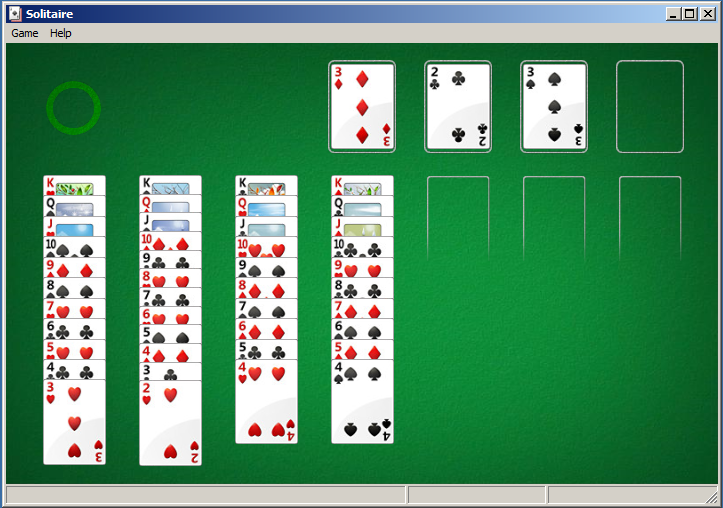
\includegraphics[width=\textwidth]{\CURPATH/1.png}}
\end{figure}

Il manque l'as de c\oe{}ur. Peut-être qu'en interne, cette carte a l'indice 51
(si les indices partent de zéro).

À un autre endroit, j'ai trouvé tous les noms des cartes. Peut-être que les noms
sont utilisés pour aller chercher l'image de la carte dans les ressources?

\begin{lstlisting}
.data:00000001000B6970 ?CARD_NAME@Card@@2PAPEBGA dq offset aTwoofclubs
.data:00000001000B6970                                         ; "TwoOfClubs"
.data:00000001000B6978                 dq offset aThreeofclubs ; "ThreeOfClubs"
.data:00000001000B6980                 dq offset aFourofclubs  ; "FourOfClubs"
.data:00000001000B6988                 dq offset aFiveofclubs  ; "FiveOfClubs"
.data:00000001000B6990                 dq offset aSixofclubs   ; "SixOfClubs"
.data:00000001000B6998                 dq offset aSevenofclubs ; "SevenOfClubs"
.data:00000001000B69A0                 dq offset aEightofclubs ; "EightOfClubs"
.data:00000001000B69A8                 dq offset aNineofclubs  ; "NineOfClubs"
.data:00000001000B69B0                 dq offset aTenofclubs   ; "TenOfClubs"
.data:00000001000B69B8                 dq offset aJackofclubs  ; "JackOfClubs"
.data:00000001000B69C0                 dq offset aQueenofclubs ; "QueenOfClubs"
.data:00000001000B69C8                 dq offset aKingofclubs  ; "KingOfClubs"
.data:00000001000B69D0                 dq offset aAceofclubs   ; "AceOfClubs"
.data:00000001000B69D8                 dq offset aTwoofdiamonds ; "TwoOfDiamonds"
.data:00000001000B69E0                 dq offset aThreeofdiamond ; "ThreeOfDiamonds"
.data:00000001000B69E8                 dq offset aFourofdiamonds ; "FourOfDiamonds"
.data:00000001000B69F0                 dq offset aFiveofdiamonds ; "FiveOfDiamonds"
.data:00000001000B69F8                 dq offset aSixofdiamonds ; "SixOfDiamonds"
.data:00000001000B6A00                 dq offset aSevenofdiamond ; "SevenOfDiamonds"
.data:00000001000B6A08                 dq offset aEightofdiamond ; "EightOfDiamonds"
.data:00000001000B6A10                 dq offset aNineofdiamonds ; "NineOfDiamonds"
.data:00000001000B6A18                 dq offset aTenofdiamonds ; "TenOfDiamonds"
.data:00000001000B6A20                 dq offset aJackofdiamonds ; "JackOfDiamonds"
.data:00000001000B6A28                 dq offset aQueenofdiamond ; "QueenOfDiamonds"
.data:00000001000B6A30                 dq offset aKingofdiamonds ; "KingOfDiamonds"
.data:00000001000B6A38                 dq offset aAceofdiamonds ; "AceOfDiamonds"
.data:00000001000B6A40                 dq offset aTwoofspades  ; "TwoOfSpades"
.data:00000001000B6A48                 dq offset aThreeofspades ; "ThreeOfSpades"
.data:00000001000B6A50                 dq offset aFourofspades ; "FourOfSpades"
.data:00000001000B6A58                 dq offset aFiveofspades ; "FiveOfSpades"
.data:00000001000B6A60                 dq offset aSixofspades  ; "SixOfSpades"
.data:00000001000B6A68                 dq offset aSevenofspades ; "SevenOfSpades"
.data:00000001000B6A70                 dq offset aEightofspades ; "EightOfSpades"
.data:00000001000B6A78                 dq offset aNineofspades ; "NineOfSpades"
.data:00000001000B6A80                 dq offset aTenofspades  ; "TenOfSpades"
.data:00000001000B6A88                 dq offset aJackofspades ; "JackOfSpades"
.data:00000001000B6A90                 dq offset aQueenofspades ; "QueenOfSpades"
.data:00000001000B6A98                 dq offset aKingofspades ; "KingOfSpades"
.data:00000001000B6AA0                 dq offset aAceofspades  ; "AceOfSpades"
.data:00000001000B6AA8                 dq offset aTwoofhearts  ; "TwoOfHearts"
.data:00000001000B6AB0                 dq offset aThreeofhearts ; "ThreeOfHearts"
.data:00000001000B6AB8                 dq offset aFourofhearts ; "FourOfHearts"
.data:00000001000B6AC0                 dq offset aFiveofhearts ; "FiveOfHearts"
.data:00000001000B6AC8                 dq offset aSixofhearts  ; "SixOfHearts"
.data:00000001000B6AD0                 dq offset aSevenofhearts ; "SevenOfHearts"
.data:00000001000B6AD8                 dq offset aEightofhearts ; "EightOfHearts"
.data:00000001000B6AE0                 dq offset aNineofhearts ; "NineOfHearts"
.data:00000001000B6AE8                 dq offset aTenofhearts  ; "TenOfHearts"
.data:00000001000B6AF0                 dq offset aJackofhearts ; "JackOfHearts"
.data:00000001000B6AF8                 dq offset aQueenofhearts ; "QueenOfHearts"
.data:00000001000B6B00                 dq offset aKingofhearts ; "KingOfHearts"
.data:00000001000B6B08                 dq offset aAceofhearts  ; "AceOfHearts"

.data:00000001000B6B10 ; public: static unsigned short const * near * Card::CARD_HUMAN_NAME
.data:00000001000B6B10 ?CARD_HUMAN_NAME@Card@@2PAPEBGA dq offset a54639Cardnames
.data:00000001000B6B10                                         ; "|54639|CardNames|Two Of Clubs"
.data:00000001000B6B18                 dq offset a64833Cardnames ; "|64833|CardNames|Three Of Clubs"
.data:00000001000B6B20                 dq offset a62984Cardnames ; "|62984|CardNames|Four Of Clubs"
.data:00000001000B6B28                 dq offset a65200Cardnames ; "|65200|CardNames|Five Of Clubs"
.data:00000001000B6B30                 dq offset a52967Cardnames ; "|52967|CardNames|Six Of Clubs"
.data:00000001000B6B38                 dq offset a42781Cardnames ; "|42781|CardNames|Seven Of Clubs"
.data:00000001000B6B40                 dq offset a49217Cardnames ; "|49217|CardNames|Eight Of Clubs"
.data:00000001000B6B48                 dq offset a44682Cardnames ; "|44682|CardNames|Nine Of Clubs"
.data:00000001000B6B50                 dq offset a51853Cardnames ; "|51853|CardNames|Ten Of Clubs"
.data:00000001000B6B58                 dq offset a46368Cardnames ; "|46368|CardNames|Jack Of Clubs"
.data:00000001000B6B60                 dq offset a61344Cardnames ; "|61344|CardNames|Queen Of Clubs"
.data:00000001000B6B68                 dq offset a65017Cardnames ; "|65017|CardNames|King Of Clubs"
.data:00000001000B6B70                 dq offset a57807Cardnames ; "|57807|CardNames|Ace Of Clubs"
.data:00000001000B6B78                 dq offset a48455Cardnames ; "|48455|CardNames|Two Of Diamonds"
.data:00000001000B6B80                 dq offset a44156Cardnames ; "|44156|CardNames|Three Of Diamonds"
.data:00000001000B6B88                 dq offset a51672Cardnames ; "|51672|CardNames|Four Of Diamonds"
.data:00000001000B6B90                 dq offset a45972Cardnames ; "|45972|CardNames|Five Of Diamonds"
.data:00000001000B6B98                 dq offset a47206Cardnames ; "|47206|CardNames|Six Of Diamonds"
.data:00000001000B6BA0                 dq offset a48399Cardnames ; "|48399|CardNames|Seven Of Diamonds"
.data:00000001000B6BA8                 dq offset a47847Cardnames ; "|47847|CardNames|Eight Of Diamonds"
.data:00000001000B6BB0                 dq offset a48606Cardnames ; "|48606|CardNames|Nine Of Diamonds"
.data:00000001000B6BB8                 dq offset a61278Cardnames ; "|61278|CardNames|Ten Of Diamonds"
.data:00000001000B6BC0                 dq offset a52038Cardnames ; "|52038|CardNames|Jack Of Diamonds"
.data:00000001000B6BC8                 dq offset a54643Cardnames ; "|54643|CardNames|Queen Of Diamonds"
.data:00000001000B6BD0                 dq offset a48902Cardnames ; "|48902|CardNames|King Of Diamonds"
.data:00000001000B6BD8                 dq offset a46672Cardnames ; "|46672|CardNames|Ace Of Diamonds"
.data:00000001000B6BE0                 dq offset a41049Cardnames ; "|41049|CardNames|Two Of Spades"
.data:00000001000B6BE8                 dq offset a49327Cardnames ; "|49327|CardNames|Three Of Spades"
.data:00000001000B6BF0                 dq offset a51933Cardnames ; "|51933|CardNames|Four Of Spades"
.data:00000001000B6BF8                 dq offset a42651Cardnames ; "|42651|CardNames|Five Of Spades"
.data:00000001000B6C00                 dq offset a65342Cardnames ; "|65342|CardNames|Six Of Spades"
.data:00000001000B6C08                 dq offset a53644Cardnames ; "|53644|CardNames|Seven Of Spades"
.data:00000001000B6C10                 dq offset a54466Cardnames ; "|54466|CardNames|Eight Of Spades"
.data:00000001000B6C18                 dq offset a56874Cardnames ; "|56874|CardNames|Nine Of Spades"
.data:00000001000B6C20                 dq offset a46756Cardnames ; "|46756|CardNames|Ten Of Spades"
.data:00000001000B6C28                 dq offset a62876Cardnames ; "|62876|CardNames|Jack Of Spades"
.data:00000001000B6C30                 dq offset a64633Cardnames ; "|64633|CardNames|Queen Of Spades"
.data:00000001000B6C38                 dq offset a46215Cardnames ; "|46215|CardNames|King Of Spades"
.data:00000001000B6C40                 dq offset a60450Cardnames ; "|60450|CardNames|Ace Of Spades"
.data:00000001000B6C48                 dq offset a51010Cardnames ; "|51010|CardNames|Two Of Hearts"
.data:00000001000B6C50                 dq offset a64948Cardnames ; "|64948|CardNames|Three Of Hearts"
.data:00000001000B6C58                 dq offset a43079Cardnames ; "|43079|CardNames|Four Of Hearts"
.data:00000001000B6C60                 dq offset a57131Cardnames ; "|57131|CardNames|Five Of Hearts"
.data:00000001000B6C68                 dq offset a58953Cardnames ; "|58953|CardNames|Six Of Hearts"
.data:00000001000B6C70                 dq offset a45105Cardnames ; "|45105|CardNames|Seven Of Hearts"
.data:00000001000B6C78                 dq offset a47775Cardnames ; "|47775|CardNames|Eight Of Hearts"
.data:00000001000B6C80                 dq offset a41825Cardnames ; "|41825|CardNames|Nine Of Hearts"
.data:00000001000B6C88                 dq offset a41501Cardnames ; "|41501|CardNames|Ten Of Hearts"
.data:00000001000B6C90                 dq offset a47108Cardnames ; "|47108|CardNames|Jack Of Hearts"
.data:00000001000B6C98                 dq offset a55659Cardnames ; "|55659|CardNames|Queen Of Hearts"
.data:00000001000B6CA0                 dq offset a44572Cardnames ; "|44572|CardNames|King Of Hearts"
.data:00000001000B6CA8                 dq offset a44183Cardnames ; "|44183|CardNames|Ace Of Hearts"
\end{lstlisting}

Si vous voulez faire ceci à quelqu'un, assurez-vous que sa santé mentale est stable.

À part les noms de fonction dans le fichier PDB, il y a de nombreux appels à la
fonction \verb|Log()| qui peuvent grandement aider,
car le jeu Solitaire signale ce qu'il est en train de faire en ce moment.

Devoir: essayer de \textit{supprimer} quelques cartes ou le deux de trèfle.
Et que se passe-t-il si nous échangeons les noms des cartes dans les tableaux de
chaînes?

J'ai aussi essayé de passer des nombres comme 0, 0..50 à \verb|Card:Init()| (pour
avoir 2 zéro dans une liste de 52 nombres).
Ainsi, j'ai vu deux cartes \textit{deux de trèfle} à un moment, mais le Solitaire
avait un comportement erratique.

Ceci est le Solitaire de Windows 7 modifié:
\href{\GitHubBlobMasterURL/examples/solitaire/51/Solitaire51.exe}{Solitaire51.exe}.


\subsection{53 cartes}

\renewcommand{\CURPATH}{examples/solitaire/53}

Maintenant, regardons la première partie de la boucle:

\begin{lstlisting}
.text:0000000100036684 loc_100036684:                          ; CODE XREF: SolitaireGame::InitialDeal(void)+C0↓j
.text:0000000100036684                 mov     eax, 4EC4EC4Fh
.text:0000000100036689                 mul     edi
.text:000000010003668B                 mov     r8d, edx
.text:000000010003668E                 shr     r8d, 4          ; unsigned int
.text:0000000100036692                 mov     eax, r8d
.text:0000000100036695                 imul    eax, 52
.text:0000000100036698                 mov     edx, edi
.text:000000010003669A                 sub     edx, eax        ; unsigned int
.text:000000010003669C                 mov     rcx, [rbx+128h] ; this
.text:00000001000366A3                 call    ?CreateCard@CardTable@@IEAAPEAVCard@@II@Z ; CardTable::CreateCard(uint,uint)
.text:00000001000366A8                 mov     rdx, rax        ; struct Card *
.text:00000001000366AB                 mov     rcx, rbx        ; this
.text:00000001000366AE                 call    ?Push@CardStack@@QEAAXPEAVCard@@@Z ; CardStack::Push(Card *)
.text:00000001000366B3                 inc     edi
.text:00000001000366B5                 cmp     edi, 52
.text:00000001000366B8                 jb      short loc_100036684
\end{lstlisting}

Qu'est-ce que cette multiplication par 4EC4EC4Fh? Il s'agit sûrement de la division
par la multiplication.
Et voici ce qu'Hex-Rays en dit:

\begin{lstlisting}
  v5 = 0;
  do
  {
    v6 = CardTable::CreateCard(v4[37], v5 % 0x34, v5 / 0x34);
    CardStack::Push((CardStack *)v4, v6);
    ++v5;
  }
  while ( v5 < 0x34 );
\end{lstlisting}

D'une certaine façon, la fonction \verb|CreateCard()| prend deux arguments:
l'itérateur divisé par 52 et le reste de l'opération de division.
Difficile de dire pourquoi ils ont fait ainsi.
Le Solitaire ne peut pas permettre plus de 52 cartes, donc le dernier argument
est absurde, il vaut toujours zéro.

Mais une fois que j'ai modifié l'instruction \TT{cmp edi, 52} en 0x1000366B5 par
\TT{cmp edi, 53}, j'ai trouvé qu'il y avait maintenant 53 cartes.
La dernière est le \textit{deux de trèfle}, car il s'agit de la carte numérotée
0.

Lors de la dernière itération, 0x52 est divisé par 0x52, le reste est zéro, donc
la carte d'indice 0 est ajoutée deux fois.

Que c'est frustrant, il y a deux \textit{deux de trèfle}:

\begin{figure}[H]
\centering
\frame{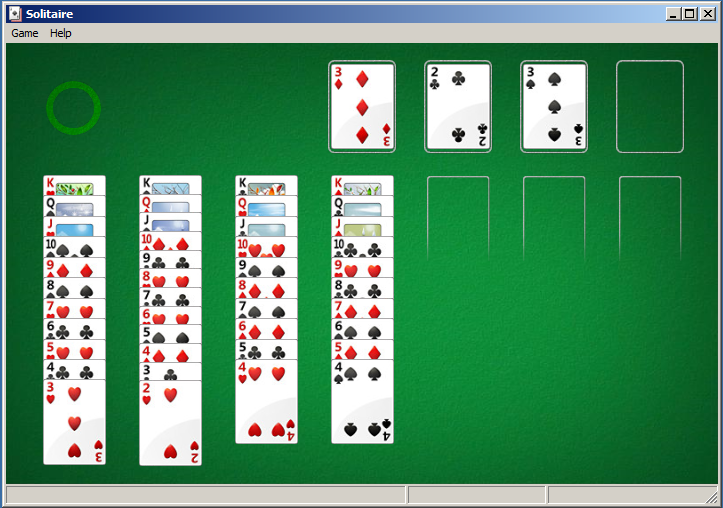
\includegraphics[width=\textwidth]{\CURPATH/1.png}}
\end{figure}

Ceci est le Solitaire de Windows 7 modifié:
\href{\RepoURL/examples/solitaire/53/Solitaire53.exe}{Solitaire53.exe}.




\mysection{Fonction presque vide}
\label{Boolector}
\myindex{Boolector}
\myindex{x86!\Instructions!JMP}

Ceci est un morceau de code réel que j'ai trouvé dans Boolector\footnote{\url{https://boolector.github.io/}}:

\lstinputlisting[style=customc]{patterns/025_almost_empty/boolectormain.c}

Pourquoi quelqu'un ferait-il comme ça?
Je ne sais pas mais mon hypothèse est que \verb|boolector_main()| peut être compilée
dans une sorte de DLL ou bibliothèque dynamique, et appelée depuis une suite de test.
Certainement qu'une suite de test peut préparer les variables argc/argv comme
le ferait \ac{CRT}.

Il est intéressant de voir comment c'est compilé:

\lstinputlisting[caption=GCC 8.2 x64 \NonOptimizing (\assemblyOutput),style=customasmx86]{patterns/025_almost_empty/boolectormain_O0.s}

Ceci est OK, le prologue (non optimisé) déplace inutilement deux arguments,
\INS{CALL}, épilogue, \INS{RET}.
Mais regardons la version optimisée:

\lstinputlisting[caption=GCC 8.2 x64 \Optimizing (\assemblyOutput),style=customasmx86]{patterns/025_almost_empty/boolectormain_O3.s}

Aussi simple que ça: la pile et les registres ne sont pas touchés et \verb|boolector_main()|
a le même ensemble d'arguments.
Donc, tout ce que nous avons à faire est de passer l'exécution à une autre adresse.

Ceci est proche d'une \glslink{thunk function}{fonction thunk}.

Nous verons queelque chose de plus avancé plus tard: \myref{ARM_B_to_printf}, \myref{JMP_instead_of_RET}.

\input{examples/qr9/qr9_FR}
% TODO translate
% TODO: OpenSSL tool, URLs, etc
\mysection{Cas de base de données chiffrée \#1}
\label{encrypted_DB1}

(Cette partie est apparue initialement dans mon blog le 26 août 2015.
Discussion: \url{https://news.ycombinator.com/item?id=10128684}.)

\subsection{Base64 et entropie}

\myindex{XML}
J'ai un fichier \ac{XML} contenant des données chiffrées.
Peut-être est-ce relatif à des commandes et/ou des information clients.

\begin{lstlisting}
<?xml version = "1.0" encoding = "UTF-8"?>
<Orders>
	<Order>
		<OrderID>1</OrderID>
		<Data>yjmxhXUbhB/5MV45chPsXZWAJwIh1S0aD9lFn3XuJMSxJ3/E+UE3hsnH</Data>
	</Order>
	<Order>
		<OrderID>2</OrderID>
		<Data>0KGe/wnypFBjsy+U0C2P9fC5nDZP3XDZLMPCRaiBw9OjIk6Tu5U=</Data>
	</Order>
	<Order>
		<OrderID>3</OrderID>
		<Data>mqkXfdzvQKvEArdzh+zD9oETVGBFvcTBLs2ph1b5bYddExzp</Data>
	</Order>
	<Order>
		<OrderID>4</OrderID>
		<Data>FCx6JhIDqnESyT3HAepyE1BJ3cJd7wCk+APCRUeuNtZdpCvQ2MR/7kLXtfUHuA==</Data>
	</Order>
...
\end{lstlisting}

Le fichier est disponible \href{\RepoURL/examples/encrypted_DB1/encrypted.xml}{ici}.

\myindex{base64}
Ce sont clairement des données encodées en base64, car toutes les chaînes consistent
en des caractères Latin, chiffres, plus (+) et symbole slash (/).
Il peut y avoir 1 ou 2 symboles de remplissage (=), mais ils ne se trouvent jamais
au milieu d'une chaîne.
Gardez à l'esprit ces propriétés du base64, il est très facile de les reconnaître.

Décodons les et calculons l'entropie (\myref{entropy}) de ces blocs dans Wolfram Mathematica:

\begin{lstlisting}
In[]:= ListOfBase64Strings =
  Map[First[#[[3]]] &, Cases[Import["encrypted.xml"], XMLElement["Data", _, _], Infinity]];

In[]:= BinaryStrings =
  Map[ImportString[#, {"Base64", "String"}] &, ListOfBase64Strings];

In[]:= Entropies = Map[N[Entropy[2, #]] &, BinaryStrings];

In[]:= Variance[Entropies]
Out[]= 0.0238614
\end{lstlisting}

\myindex{Variance}
La variance est basse.
Cela signifie que l'entropie des valeurs ne sont pas très différentes les unes des autres.
Ceci est visible sur le graphique:

\begin{lstlisting}
In[]:= ListPlot[Entropies]
\end{lstlisting}

\begin{figure}[H]
\centering
\myincludegraphics{examples/encrypted_DB1/entropy.png}
\end{figure}

La plupart des valeurs sont entre 5.0 et 5.4.
Ceci est un signe que les données sont compressées et/ou chiffrées

Pour comprendre la variance, calculons l'entropie de toutes les liens du livre de
Conan Doyle \emph{The Hound of the Baskervilles}:

\begin{lstlisting}
In[]:= BaskervillesLines = Import["http://www.gutenberg.org/cache/epub/2852/pg2852.txt", "List"];

In[]:= EntropiesT = Map[N[Entropy[2, #]] &, BaskervillesLines];

In[]:= Variance[EntropiesT]
Out[]= 2.73883

In[]:= ListPlot[EntropiesT]
\end{lstlisting}

\begin{figure}[H]
\centering
\myincludegraphics{examples/encrypted_DB1/conan_doyle.png}
\end{figure}

La plupart des valeurs sont regroupées autour de 4, mais il y a aussi des valeurs
qui sont plus petites, et elles influencent la valeur finale de la variance.

Peut-être que les chaînes courtes ont une entropie plus petite, prenons les chaînes
courtes du livre de Conan Doyle.

\begin{lstlisting}
In[]:= Entropy[2, "Yes, sir."] // N
Out[]= 2.9477
\end{lstlisting}

Essayons encore plus petit:

\begin{lstlisting}
In[]:= Entropy[2, "Yes"] // N
Out[]= 1.58496

In[]:= Entropy[2, "No"] // N
Out[]= 1.
\end{lstlisting}

\subsection{Est-ce que les données sont compressées?}

OK, donc nos données sont compressées et/ou chiffrées.
Sont-elles compressées? Presque tous les compresseurs de données ajoutent un entête
au début, une signature ou quelque chose comme ça.
Comme on peut le voir, il n'y a pas de motifs communs au début de chaque bloc.
Il est toujours possible qu'il s'agisse d'un compresseur de données écrit à la main,
mais c'est très rare.
D'un autre côté, les algorithmes de chiffrement maison sont plus répandus, car il
est facile d'en faire un.
\myindex{memfrob()}
\myindex{ROT13}
Même des systèmes de chiffrement sans clef primitifs comme \emph{memfrob()}\footnote{\url{http://linux.die.net/man/3/memfrob}}
et ROT13 fonctionnent bien sans erreur.
C'est un gros défi d'écrire un compresseur depuis zéro, en utilisant seulement sa
fantaisie et son imagination de façon à ce qu'il n'ait pas de bugs évidents.
Certains programmeurs implémentent des fonctions de compression de données en lisant
des livres, mais ceci est aussi rare.
Les deux moyens les plus fréquents sont:
\myindex{zlib}
1) utiliser simplement la bibliothèque open-source zlib;
2) copier/coller quelque chose de quelque part.
Les algorithmes de compression open-source mettent en général une sorte d'en-tête,
ainsi que les algorithmes de sites comme \url{http://www.codeproject.com/}.

\subsection{Est-ce que les données sont chiffrées?}

Les algorithmes majeurs de chiffrement de données traitent les données par bloc.
DES---8 octets, AES---16 octets. 
Si le buffer en entrée n'est pas divisible par la taille du bloc, des zéros sont
ajoutés (ou quelque chose d'autre), afin que les donnés chiffrées soient alignées
sur la taille du bloc de l'algorithme.
Ce n'est pas notre cas.

En utilisant Wolfram Mathematica, j'ai analysé la longueur des blocs:

\begin{lstlisting}
In[]:= Counts[Map[StringLength[#] &, BinaryStrings]]
Out[]= <|42 -> 1858, 38 -> 1235, 36 -> 699, 46 -> 1151, 40 -> 1784,
 44 -> 1558, 50 -> 366, 34 -> 291, 32 -> 74, 56 -> 15, 48 -> 716,
 30 -> 13, 52 -> 156, 54 -> 71, 60 -> 3, 58 -> 6, 28 -> 4|>
\end{lstlisting}

1858 blocs ont une taille de 42 octets, 1235 blocs ont une taille de 38 octets, etc.

J'ai fait un graphe:

\begin{lstlisting}
ListPlot[Counts[Map[StringLength[#] &, BinaryStrings]]]
\end{lstlisting}

\begin{figure}[H]
\centering
\myincludegraphics{examples/encrypted_DB1/lengths.png}
\end{figure}

Donc, la plupart des blocs ont une taille entre $\textasciitilde{}36$ et $\textasciitilde{}48$.
Il y a un autre chose à remarquer: tous les blocs ont une taille paire.
Pas un bloc n'a une taille impaire.

Il y a, toutefois, des flux de chiffrement qui opèrent au niveau de l'octet ou même
du bit.

\subsection{CryptoPP}
\myindex{CryptoPP}

Le programme qui peut parcourir cette base de données chiffrées est écrit en C\#
et le code .NET est fortement obscurci.
Néanmoins, il y a une DLL avec du code x86, qui, après un bref examen, contient des
parties de la bibliothèque open-source connue CryptoPP!
(J'ai juste repéré des chaînes \q{CryptoPP} dedans.)
Maintenant, c'est très facile de trouver toutes les fonctions à l'intérieur de la
DLL car la bibliothèque CryptoPP est open-source.

\myindex{AES}
La bibliothèque CryptoPP contient beaucoup de fonctions de chiffrement, AES inclus (AKA Rijndael).
Les CPUs x86 récents possèdent des instructions dédiées à AES comme \INS{AESENC}, \INS{AESDEC}
et \INS{AESKEYGENASSIST}\footnote{\url{https://en.wikipedia.org/wiki/AES_instruction_set}}.
Elles ne font pas le chiffrement/déchiffrement complètement, mais elles font une
part significative du travail.
Et les nouvelles versions de CryptoPP les utilisent.
Par exemple, ici:
\href{https://github.com/mmoss/cryptopp/blob/2772f7b57182b31a41659b48d5f35a7b6cedd34d/src/rijndael.cpp#L1034}{1},
\href{https://github.com/mmoss/cryptopp/blob/2772f7b57182b31a41659b48d5f35a7b6cedd34d/src/rijndael.cpp#L1000}{2}.
\myindex{x86!\Instructions!AESENC}
\myindex{x86!\Instructions!AESDEC}
\myindex{tracer}
À ma surprise, lors du déchiffrement, \INS{AESENC} est exécutée, tandis que \INS{AESDEC}
ne l'est pas (j'ai vérifié avec mon utilitaire tracer, mais n'importe quel débogueur
peut être utilisé).
J'ai vérifié, si mon CPU supporte réellement les instructions AES. Certains CPUs
Intel i3 ne les supportent pas.
Et si non, la bibliothèque CryptoPP se rabat sur les fonctions implémentées de l'ancienne façon
\footnote{\url{https://github.com/mmoss/cryptopp/blob/2772f7b57182b31a41659b48d5f35a7b6cedd34d/src/rijndael.cpp#L355}}.
Mais mon CPU les supporte.
Pourquoi \INS{AESDEC} n'est pas exécuté?
Pourquoi le programme utilise le chiffrement AES pour déchiffrer la base de données?

OK, ce n'est pas un problème de trouver la fonction qui chiffre les blocs.
Elle est appelée \\
\emph{CryptoPP::Rijndael::Enc::ProcessAndXorBlock}:
\href{https://github.com/mmoss/cryptopp/blob/2772f7b57182b31a41659b48d5f35a7b6cedd34d/src/rijndael.cpp#L349}{src},
et elle peut être appelée depuis une autre fonction: \\
\emph{Rijndael::Enc::AdvancedProcessBlocks()}
\href{https://github.com/mmoss/cryptopp/blob/2772f7b57182b31a41659b48d5f35a7b6cedd34d/src/rijndael.cpp#L1179}{src},
qui, à son tour, appelle les deux fonctions: (
\href{https://github.com/mmoss/cryptopp/blob/2772f7b57182b31a41659b48d5f35a7b6cedd34d/src/rijndael.cpp#L1000}{AESNI\_Enc\_Block}
et
\href{https://github.com/mmoss/cryptopp/blob/2772f7b57182b31a41659b48d5f35a7b6cedd34d/src/rijndael.cpp#L1012}{AESNI\_Enc\_4\_Blocks}
)
qui ont les instructions  \INS{AESENC}.

Donc, a en juger par les entrailles de CryptoPP \\
\emph{CryptoPP::Rijndael::Enc::ProcessAndXorBlock()} chiffre un bloc 16-octet.
Mettons un point d'arrêt dessus et voyons ce qui se produit pendant le déchiffrement.
J'utilise à nouveau mon petit outil tracer.
Le logiciel doit déchiffrer le premier bloc de données maintenant.
Oh, à propos, voici le premier bloc de données converti de l'encodage en base64 vers
des données hexadécimale, faisons le manuellement:

\lstinputlisting{examples/encrypted_DB1/1.lst}

Voici les arguments de la fonction d'après les fichiers sources de CryptoPP:

\begin{lstlisting}
size_t Rijndael::Enc::AdvancedProcessBlocks(const byte *inBlocks, const byte *xorBlocks, byte *outBlocks, size_t length, word32 flags);
\end{lstlisting}

Donc, il y a 5 arguments. Les flags possibles sont:

\begin{lstlisting}
enum {BT_InBlockIsCounter=1, BT_DontIncrementInOutPointers=2, BT_XorInput=4, BT_ReverseDirection=8, BT_AllowParallel=16} FlagsForAdvancedProcessBlocks;
\end{lstlisting}

OK, lançons tracer sur la fonction \emph{ProcessAndXorBlock()}:

\lstinputlisting{examples/encrypted_DB1/2.lst}

Ici nous pouvons voir l'entrée de la fonction \emph{ProcessAndXorBlock()}, et sa sortie.

Ceci est la sortie de la fonction lors du premier appel:

\begin{lstlisting}
00000000: C7 39 4E 7B 33 1B D6 1F-B8 31 10 39 39 13 A5 5D ".9N{3....1.99..]"
\end{lstlisting}

Puis la fonction \emph{ProcessAndXorBlock()} est appelée avec un bloc de longueur
zéro, mais avec le flag 8 (\emph{BT\_ReverseDirection}).

Second appel:

\begin{lstlisting}
00000000: 45 00 20 00 4A 00 4F 00-48 00 4E 00 53 00 00 00 "E. .J.O.H.N.S..."
\end{lstlisting}

Maintenant, il y a des chaînes qui nous sont familières!

Troisième appel:

\begin{lstlisting}
00000000: B1 27 7F E4 9F 01 E3 81-CF C6 12 FB B9 7C F1 BC ".'...........|.."
\end{lstlisting}

La première sortie est très similaire aux 16 premiers octets du buffer chiffré.

Sortie du premier appel à \emph{ProcessAndXorBlock()}:

\begin{lstlisting}
00000000: C7 39 4E 7B 33 1B D6 1F-B8 31 10 39 39 13 A5 5D ".9N{3....1.99..]"
\end{lstlisting}

16 premiers octets du buffer chiffré:

\begin{lstlisting}
00000000: CA 39 B1 85 75 1B 84 1F F9 31 5E 39 72 13 EC 5D  .9..u....1^9r..]
\end{lstlisting}

Il y a trop d'octets égaux!
Comment le résultat du chiffrement AES peut-il être aussi similaire au buffer chiffré
alors que ceci n'est pas du chiffrement mais bien du déchiffrement?!

\subsection{Mode Cipher Feedback}

\myindex{Cipher Feedback mode}
\myindex{XOR}
La réponse est \ac{CFB}:
Dans ce mode, l'algorithme AES n'est pas utilisé comme un algorithme de chiffrement,
mais comme un dispositif qui génère des données aléatoires cryptographiquement sûres.
Le chiffrement effectif est obtenu en utilisant une simple opération XOR.

Voici l'algorithme de chiffrement (les images proviennent de Wikipédia):

\begin{figure}[H]
\centering
\myincludegraphics{examples/encrypted_DB1/601px-CFB_encryption.png}
\end{figure}

Et le déchiffrement:

\begin{figure}[H]
\centering
\myincludegraphics{examples/encrypted_DB1/601px-CFB_decryption.png}
\label{fig:CFB_decryption}
\end{figure}

Maintenant regardons: le chiffrement AES génère 16 octets (ou 128 bits) de données
\emph{aléatoires} destinées à être utilisées lors du XOR, qui nous oblige à utiliser
tous les 16 octets?
Si à la dernière itération nous n'avons qu'un octet de données, nous ne chiffrons
qu'un octet avec un octet de données \emph{aléatoires} générée.
Ceci conduit à une propriété importante du mode \ac{CFB}: les données ne doivent
pas être adaptées à une taille, des données de taille arbitraire peuvent être chiffrées
et déchiffrées.

Oh, c'est pour ça que les blocs chiffrés ne sont pas complétés.
Et c'est pourquoi l'instruction \INS{AESDEC} n'est jamais appelée.

Essayons de déchiffrer le premier bloc manuellement, en utilisant Python.
Le mode \ac{CFB} utilise aussi un \ac{IV}, comme \emph{semence} pour \ac{CSPRNG}.
Dans notre cas, l'\ac{IV} est le bloc qui est chiffré à la première itération:

\begin{lstlisting}
0038B920: 01 00 00 00 FF FF FF FF-79 C1 69 0B 67 C1 04 7D "........y.i.g..}"
\end{lstlisting}

Oh, et nous devons aussi retrouver la clef de chiffrement.
\myindex{x86!\Instructions!AESKEYGENASSIST}
Il y a \INS{AESKEYGENASSIST} dans la DLL, et elle est appelée, et elle est utilisée dans la fonction \\
\href{https://github.com/mmoss/cryptopp/blob/2772f7b57182b31a41659b48d5f35a7b6cedd34d/src/rijndael.cpp#L198}{src}.
C'est facile de la trouver dans \IDA et de mettre un point d'arrêt. Voyons:

\begin{lstlisting}
... tracer.exe -l:filename.exe bpf=filename.exe!0x435c30,args:3,dump_args:0x10

Warning: no tracer.cfg file.
PID=2068|New process software.exe
no module registered with image base 0x77320000
no module registered with image base 0x76e20000
no module registered with image base 0x77320000
no module registered with image base 0x77220000
Warning: unknown (to us) INT3 breakpoint at ntdll.dll!LdrVerifyImageMatchesChecksum+0x96c (0x776c103b)
(0) software.exe!0x435c30(0x15e8000, 0x10, 0x14f808) (called from software.exe!.text+0x22fa1 (0x13d3fa1))
Argument 1/3
015E8000: CD C5 7E AD 28 5F 6D E1-CE 8F CC 29 B1 21 88 8E "..~.(_m....).!.."
Argument 3/3
0014F808: 38 82 58 01 C8 B9 46 00-01 D1 3C 01 00 F8 14 00 "8.X...F...<....."
Argument 3/3 +0x0: software.exe!.rdata+0x5238
Argument 3/3 +0x8: software.exe!.text+0x1c101
(0) software.exe!0x435c30() -> 0x13c2801
PID=2068|Process software.exe exited. ExitCode=0 (0x0)
\end{lstlisting}

Donc, ceci est la clef: \emph{CD C5 7E AD 28 5F 6D E1-CE 8F CC 29 B1 21 88 8E}.

Durant le déchiffrement manuel, nous obtenons ceci:

\begin{lstlisting}
00000000: 0D 00 FF FE 46 00 52 00  41 00 4E 00 4B 00 49 00  ....F.R.A.N.K.I.
00000010: 45 00 20 00 4A 00 4F 00  48 00 4E 00 53 00 66 66  E. .J.O.H.N.S.ff
00000020: 66 66 66 9E 61 40 D4 07  06 01                    fff.a@....
\end{lstlisting}

Maintenant, c'est quelque chose de lisible!
Et nous comprenons pourquoi il y avait autant d'octets égaux dans la première
itération de déchiffrement:
car le text en clair a beaucoup d'octet à zéro!
Déchiffrons le second bloc:

\begin{lstlisting}
00000000: 17 98 D0 84 3A E9 72 4F  DB 82 3F AD E9 3E 2A A8  ....:.rO..?..>*.
00000010: 41 00 52 00 52 00 4F 00  4E 00 CD CC CC CC CC CC  A.R.R.O.N.......
00000020: 1B 40 D4 07 06 01                                 .@....
\end{lstlisting}

Les troisième, quatrième et cinquième:

\begin{lstlisting}
00000000: 5D 90 59 06 EF F4 96 B4  7C 33 A7 4A BE FF 66 AB  ].Y.....|3.J..f.
00000010: 49 00 47 00 47 00 53 00  00 00 00 00 00 C0 65 40  I.G.G.S.......e@
00000020: D4 07 06 01                                       ....
\end{lstlisting}

\begin{lstlisting}
00000000: D3 15 34 5D 21 18 7C 6E  AA F8 2D FE 38 F9 D7 4E  ..4]!.|n..-.8..N
00000010: 41 00 20 00 44 00 4F 00  48 00 45 00 52 00 54 00  A. .D.O.H.E.R.T.
00000020: 59 00 48 E1 7A 14 AE FF  68 40 D4 07 06 02        Y.H.z...h@....
\end{lstlisting}

\begin{lstlisting}
00000000: 1E 8B 90 0A 17 7B C5 52  31 6C 4E 2F DE 1B 27 19  .....{.R1lN...'.
00000010: 41 00 52 00 43 00 55 00  53 00 00 00 00 00 00 60  A.R.C.U.S.......
00000020: 66 40 D4 07 06 03                                 f@....
\end{lstlisting}

Tous les blocs déchiffrés semblent correct, à l'exception des 16 premiers octets.

\subsection{Initializing Vector}

Qu'est-ce qui peut affecter les 16 premiers octets?

Revenons à nouveau à l'algorithme de déchiffrement \ac{CFB}: \myref{fig:CFB_decryption}.

Nous pouvons voir que l'\ac{IV} peut affecter le déchiffrement de la première opération
de déchiffrement, mais pas la seconde, car lors de la seconde itération, le texte
chiffré de la première itération est utilisé, et en cas de déchiffrement, c'est le
même, quelque soit l'\ac{IV}!

Donc, l'\ac{IV} est sans doute différent à chaque fois.
En utilisant mon tracer, j'ai regardé la première entrée lors du déchiffrement du
second bloc du fichier \ac{XML}:

\begin{lstlisting}
0038B920: 02 00 00 00 FE FF FF FF-79 C1 69 0B 67 C1 04 7D "........y.i.g..}"
\end{lstlisting}

\dots troisième:

\begin{lstlisting}
0038B920: 03 00 00 00 FD FF FF FF-79 C1 69 0B 67 C1 04 7D "........y.i.g..}"
\end{lstlisting}

Il semble que le premier et le cinquième octet changent à chaque fois.
J'en ai finalement conclu que le premier entier 32-bit est simplement OrderID du fichier
\ac{XML}, et le second entier 32-bit est aussi OrderID, mais multiplié par -1. Tous
les 8 autres octets sont les mêmes pour chaque opération.
Maintenant, j'ai déchiffré la base de données entière:
\url{\RepoURL/examples/encrypted_DB1/decrypted.full.txt}.

Le script Python utilisé pour ceci est:
\url{\RepoURL/examples/encrypted_DB1/decrypt_blocks.py}.

Peut-être que l'auteur voulait chiffrer chaque bloc différemment, donc il a utilisé
OrderID comme une partie de la clef.
Il aurait aussi été possible de créer une clef AES différente, au lieu de l'\ac{IV}.

Dinc maintenant nous savons que l'\ac{IV} affecte seulement le premier bloc lors
du déchiffrement en mode \ac{CFB}, ceci en est une caractéristique.
Tous les autres blocs peuvent être déchiffrés sans connaître l'\ac{IV}, mais en utilisant
la clef.

OK, donc pourquoi le mode \ac{CFB}? Apparemment, parce que le tout premier exemple
sur le wiki de CryptoPP utilise le mode \ac{CFB}:
\url{http://www.cryptopp.com/wiki/Advanced_Encryption_Standard#Encrypting_and_Decrypting_Using_AES}.
On peut aussi supposer que le développeur l'a choisi pour sa simplicité:
l'exemple peut chiffrer/déchiffrer des chaînes de texte de longueur arbitraire, sans
remplissage.

Il est aussi probable que l'auteur du programme a juste copié/collé l'exemple depuis
la page wiki de CryptoPP.
Beaucoup de programmeurs font ça.

La seule différence est que l'\ac{IV} est choisi aléatoirement dans l'exemple du
wiki de CryptoPP, alors que cet indéterminisme n'était pas permis aux programmeurs
du logiciel que nous disséquons maintenant, donc ils ont choisi d'initialiser l'\ac{IV}
en utilisant OrderID.

Nous pouvons maintenant procéder à l'analyse du cas de chaque octet dans le bloc
déchiffré.

\subsection{Structure du buffer}

Prenons les quatre premier bloc déchiffrés:

\begin{lstlisting}
00000000: 0D 00 FF FE 46 00 52 00  41 00 4E 00 4B 00 49 00  ....F.R.A.N.K.I.
00000010: 45 00 20 00 4A 00 4F 00  48 00 4E 00 53 00 66 66  E. .J.O.H.N.S.ff
00000020: 66 66 66 9E 61 40 D4 07  06 01                    fff.a@....

00000000: 0B 00 FF FE 4C 00 4F 00  52 00 49 00 20 00 42 00  ....L.O.R.I. .B.
00000010: 41 00 52 00 52 00 4F 00  4E 00 CD CC CC CC CC CC  A.R.R.O.N.......
00000020: 1B 40 D4 07 06 01                                 .@....

00000000: 0A 00 FF FE 47 00 41 00  52 00 59 00 20 00 42 00  ....G.A.R.Y. .B.
00000010: 49 00 47 00 47 00 53 00  00 00 00 00 00 C0 65 40  I.G.G.S.......e@
00000020: D4 07 06 01                                       ....

00000000: 0F 00 FF FE 4D 00 45 00  4C 00 49 00 4E 00 44 00  ....M.E.L.I.N.D.
00000010: 41 00 20 00 44 00 4F 00  48 00 45 00 52 00 54 00  A. .D.O.H.E.R.T.
00000020: 59 00 48 E1 7A 14 AE FF  68 40 D4 07 06 02        Y.H.z...h@....
\end{lstlisting}

On voit clairement des chaînes de textes encodées en UTF-16, ce sont les noms et
noms de famille.
Le premier octet (ou mot de 16-bit) semble être la longueur de la chaîne, nous pouvons
vérifier visuellement.
\emph{FF FE} semble être le \ac{BOM} Unicode.

Il y a 12 autres octets après chaque chaîne.

En utilisant ce script
(\url{\RepoURL/examples/encrypted_DB1/dump_buffer_rest.py})
j'ai obtenu une sélection aléatoire de \emph{fins} (de bloc):

\lstinputlisting{examples/encrypted_DB1/tails.lst}

Nous voyons tout d'abord que les octets 0x40 et 0x07 sont présent dans chaque \emph{fin}.
Le tout dernier octet est toujours dans l'intervalle 1..0x1F (1..31), j'ai vérifié.
Le pénultième octet est toujours dans l'intervalle 1..0xC (1..12).
Ouah, ça ressemble à une date!
L'année peut être représentée comme une valeur 16-bit, et peut-être que les 4 derniers
octets sont une date (16 bits pour l'année, 8 bits pour le mois et les 8 restants
pour le jour)?
0x7DD est 2013, 0x7D5 est 2005, etc. Ça semble juste. Ceci est une date.
Il y a 8 octets supplémentaires.
À en juger par le fait que ceci est une base de données appelée \emph{orders}, peut-être
s'agit-il d'une sorte de somme ici?
J'ai essayé de les interpréter comme des réels en double précision IEEE 754 et ai
affiché toutes les valeurs!

Certaines sont:

\begin{lstlisting}
71.0
134.0
51.95
53.0
121.99
96.95
98.95
15.95
85.95
184.99
94.95
29.95
85.0
36.0
130.99
115.95
87.99
127.95
114.0
150.95
\end{lstlisting}

Ça ressemble à des nombres réels

Maintenant, nous pouvons afficher les noms, sommes et dates.

\begin{lstlisting}
plain:
00000000: 0D 00 FF FE 46 00 52 00  41 00 4E 00 4B 00 49 00  ....F.R.A.N.K.I.
00000010: 45 00 20 00 4A 00 4F 00  48 00 4E 00 53 00 66 66  E. .J.O.H.N.S.ff
00000020: 66 66 66 9E 61 40 D4 07  06 01                    fff.a@....
OrderID= 1 name= FRANKIE JOHNS sum= 140.95 date= 2004 / 6 / 1

plain:
00000000: 0B 00 FF FE 4C 00 4F 00  52 00 49 00 20 00 42 00  ....L.O.R.I. .B.
00000010: 41 00 52 00 52 00 4F 00  4E 00 CD CC CC CC CC CC  A.R.R.O.N.......
00000020: 1B 40 D4 07 06 01                                 .@....
OrderID= 2 name= LORI BARRON sum= 6.95 date= 2004 / 6 / 1

plain:
00000000: 0A 00 FF FE 47 00 41 00  52 00 59 00 20 00 42 00  ....G.A.R.Y. .B.
00000010: 49 00 47 00 47 00 53 00  00 00 00 00 00 C0 65 40  I.G.G.S.......e@
00000020: D4 07 06 01                                       ....
OrderID= 3 name= GARY BIGGS sum= 174.0 date= 2004 / 6 / 1

plain:
00000000: 0F 00 FF FE 4D 00 45 00  4C 00 49 00 4E 00 44 00  ....M.E.L.I.N.D.
00000010: 41 00 20 00 44 00 4F 00  48 00 45 00 52 00 54 00  A. .D.O.H.E.R.T.
00000020: 59 00 48 E1 7A 14 AE FF  68 40 D4 07 06 02        Y.H.z...h@....
OrderID= 4 name= MELINDA DOHERTY sum= 199.99 date= 2004 / 6 / 2

plain:
00000000: 0B 00 FF FE 4C 00 45 00  4E 00 41 00 20 00 4D 00  ....L.E.N.A. .M.
00000010: 41 00 52 00 43 00 55 00  53 00 00 00 00 00 00 60  A.R.C.U.S.......
00000020: 66 40 D4 07 06 03                                 f@....
OrderID= 5 name= LENA MARCUS sum= 179.0 date= 2004 / 6 / 3
\end{lstlisting}

En voir plus: \url{\RepoURL/examples/encrypted_DB1/decrypted.full.with_data.txt}.
Ou filtré: \url{\RepoURL/examples/encrypted_DB1/decrypted.short.txt}.
Ça semble correct.

Ceci est une sorte de sérialisation \ac{OOP}, i.e., stockant différents types de
valeurs dans un buffer binaire pour le stocker et/ou le transmettre.

\subsection{Bruit en fin de buffer}

La seule question qui reste est que, parfois, la \emph{fin} est plus longue:

\begin{lstlisting}
00000000: 0E 00 FF FE 54 00 48 00  45 00 52 00 45 00 53 00  ....T.H.E.R.E.S.
00000010: 45 00 20 00 54 00 55 00  54 00 54 00 4C 00 45 00  E. .T.U.T.T.L.E.
00000020: 66 66 66 66 66 1E 63 40  D4 07 07 1A 00 07 07 19  fffff.c@........
OrderID= 172 name= THERESE TUTTLE sum= 152.95 date= 2004 / 7 / 26
\end{lstlisting}

(Les octets \emph{00 07 07 19} ne sont pas utilisés et servent de remplissage.)

\begin{lstlisting}
00000000: 0C 00 FF FE 4D 00 45 00  4C 00 41 00 4E 00 49 00  ....M.E.L.A.N.I.
00000010: 45 00 20 00 4B 00 49 00  52 00 4B 00 00 00 00 00  E. .K.I.R.K.....
00000020: 00 20 64 40 D4 07 09 02  00 02                    . d@......
OrderID= 286 name= MELANIE KIRK sum= 161.0 date= 2004 / 9 / 2
\end{lstlisting}

(\emph{00 02} ne sont pas utilisés.)

Après un examen rigoureux, on peut voir que le but à la fin de la \emph{fin} est
juste le reste d'un chiffrement précédent!

Voici deux buffers consécutifs:

\begin{lstlisting}
00000000: 10 00 FF FE 42 00 4F 00  4E 00 4E 00 49 00 45 00  ....B.O.N.N.I.E.
00000010: 20 00 47 00 4F 00 4C 00  44 00 53 00 54 00 45 00   .G.O.L.D.S.T.E.
00000020: 49 00 4E 00 9A 99 99 99  99 79 46 40 D4 07 07 19  I.N......yF@....
OrderID= 171 name= BONNIE GOLDSTEIN sum= 44.95 date= 2004 / 7 / 25

00000000: 0E 00 FF FE 54 00 48 00  45 00 52 00 45 00 53 00  ....T.H.E.R.E.S.
00000010: 45 00 20 00 54 00 55 00  54 00 54 00 4C 00 45 00  E. .T.U.T.T.L.E.
00000020: 66 66 66 66 66 1E 63 40  D4 07 07 1A 00 07 07 19  fffff.c@........
OrderID= 172 name= THERESE TUTTLE sum= 152.95 date= 2004 / 7 / 26
\end{lstlisting}

(Les derniers octets \emph{07 07 19} sont copiés du buffer précédent.) 

Un autre exemple de deux buffers consécutifs:

\begin{lstlisting}
00000000: 0D 00 FF FE 4C 00 4F 00  52 00 45 00 4E 00 45 00  ....L.O.R.E.N.E.
00000010: 20 00 4F 00 54 00 4F 00  4F 00 4C 00 45 00 CD CC   .O.T.O.O.L.E...
00000020: CC CC CC 3C 5E 40 D4 07  09 02                    ...<^@....
OrderID= 285 name= LORENE OTOOLE sum= 120.95 date= 2004 / 9 / 2

00000000: 0C 00 FF FE 4D 00 45 00  4C 00 41 00 4E 00 49 00  ....M.E.L.A.N.I.
00000010: 45 00 20 00 4B 00 49 00  52 00 4B 00 00 00 00 00  E. .K.I.R.K.....
00000020: 00 20 64 40 D4 07 09 02  00 02                    . d@......
OrderID= 286 name= MELANIE KIRK sum= 161.0 date= 2004 / 9 / 2
\end{lstlisting}

Le dernier octet 02 a été copié du buffer en texte clair précédent.

C'est possible si le buffer utilisé lors du chiffrement est global et/ou s'il n'est
pas mis à zéro entre chaque chiffrement.
La taille du buffer final est aussi chaotique, néanmoins, le bogue reste sans conséquence
car il n'affecte pas le processus de déchiffrement, qui ignore le bruit à la fin.
C'est une erreur courante.
\myindex{OpenSSL}
\myindex{Heartbleed}
Il était présent dans OpenSSL (Heartbleed bug).

\subsection{Conclusion}

Résumé:
Chaque rétro-ingénieur pratiquant doit être familier avec la majorité des algorithmes
ainsi que la majorité des modes de chiffrement.
Quelques livres à ce sujet: \myref{crypto_books}.

Le contenu \emph{chiffré} de la base de données a été artificiellement construit
par moi, pour les besoins de la démonstration.
J'ai obtenu les nom et noms de famille les plus répandus au USA ici: \url{http://stackoverflow.com/questions/1803628/raw-list-of-person-names},
et les ai combiné aléatoirement.
Les dates et montants ont aussi été générés aléatoirement.

Tous les fichiers utilisés dans cette partie sont ici: \url{\RepoURL/examples/encrypted_DB1}.

Néanmoins, j'ai observé de telles caractéristiques dans des logiciels réels.
Cet exemple est basé dessus.

\subsection{Post Scriptum: brute-force \ac{IV}}

Le cas que vous venez de voir a été construit artificiellement, mais il est basé
sur des logiciels réels que j'ai rétro-ingénièré.
Lorsque j'ai travaillé dessus, j'ai d'abord remarqué que l'\ac{IV} avait été généré
en utilisant un nombre 32-bit, et je n'ai pas été capable de trouver un lien entre
cette valeur et OrderID.
Donc j'ai utilisé le brute-force, ce qui est aussi possible ici.

Ce n'est pas un problème d'énumérer toutes les valeurs 32-bit et d'essayer chacune
d'elle comme base pour l'\ac{IV}.
Ensuite vous déchiffrez le premier bloc de 16 octets et vérifiez les octets à zéro,
qui sont toujours à des places fixes.

\mysection{Overclocker le mineur de Bitcoin Cointerra}
\myindex{Bitcoin}
\myindex{BeagleBone}

Il y avait le mineur de Bitcoin Cointerra, ressemblant à ceci:

\begin{figure}[H]
\centering
\myincludegraphics{examples/bitcoin_miner/board.jpg}
\caption{Carte}
\end{figure}

Et il y avait aussi (peut-être leaké) l'utilitaire\footnote{Peut être téléchargé ici: \url{\RepoURL/examples/bitcoin_miner/files/cointool-overclock}}
qui peut définir la fréquence d'horloge pour la carte.
Il fonctionne sur une carte additionnelle BeagleBone Linux ARM (petite carte en bas
de l'image).

Et on m'avait demandé une fois s'il est possible de modifier cet utilitaire pour voir
quelles sont les fréquences qui peuvent être définies, et celles qui ne peuvent pas
l'être.
Et est-il possible de l'ajuster?

L'utilitaire doit être exécuté comme cela: \TT{./cointool-overclock 0 0 900}, où 900
est la fréquence en MHz.
Si la fréquence est trop grande, l'utilitaire affiche \q{Error with arguments} et
se termine.

Ceci est le morceau de code autour de la référence à la chaîne de texte \q{Error with arguments}:

\begin{lstlisting}[style=customasmARM]

...

.text:0000ABC4         STR      R3, [R11,#var_28]
.text:0000ABC8         MOV      R3, #optind
.text:0000ABD0         LDR      R3, [R3]
.text:0000ABD4         ADD      R3, R3, #1
.text:0000ABD8         MOV      R3, R3,LSL#2
.text:0000ABDC         LDR      R2, [R11,#argv]
.text:0000ABE0         ADD      R3, R2, R3
.text:0000ABE4         LDR      R3, [R3]
.text:0000ABE8         MOV      R0, R3  ; nptr
.text:0000ABEC         MOV      R1, #0  ; endptr
.text:0000ABF0         MOV      R2, #0  ; base
.text:0000ABF4         BL       strtoll
.text:0000ABF8         MOV      R2, R0
.text:0000ABFC         MOV      R3, R1
.text:0000AC00         MOV      R3, R2
.text:0000AC04         STR      R3, [R11,#var_2C]
.text:0000AC08         MOV      R3, #optind
.text:0000AC10         LDR      R3, [R3]
.text:0000AC14         ADD      R3, R3, #2
.text:0000AC18         MOV      R3, R3,LSL#2
.text:0000AC1C         LDR      R2, [R11,#argv]
.text:0000AC20         ADD      R3, R2, R3
.text:0000AC24         LDR      R3, [R3]
.text:0000AC28         MOV      R0, R3  ; nptr
.text:0000AC2C         MOV      R1, #0  ; endptr
.text:0000AC30         MOV      R2, #0  ; base
.text:0000AC34         BL       strtoll
.text:0000AC38         MOV      R2, R0
.text:0000AC3C         MOV      R3, R1
.text:0000AC40         MOV      R3, R2
.text:0000AC44         STR      R3, [R11,#third_argument]
.text:0000AC48         LDR      R3, [R11,#var_28]
.text:0000AC4C         CMP      R3, #0
.text:0000AC50         BLT      errors_with_arguments
.text:0000AC54         LDR      R3, [R11,#var_28]
.text:0000AC58         CMP      R3, #1
.text:0000AC5C         BGT      errors_with_arguments
.text:0000AC60         LDR      R3, [R11,#var_2C]
.text:0000AC64         CMP      R3, #0
.text:0000AC68         BLT      errors_with_arguments
.text:0000AC6C         LDR      R3, [R11,#var_2C]
.text:0000AC70         CMP      R3, #3
.text:0000AC74         BGT      errors_with_arguments
.text:0000AC78         LDR      R3, [R11,#third_argument]
.text:0000AC7C         CMP      R3, #0x31
.text:0000AC80         BLE      errors_with_arguments
.text:0000AC84         LDR      R2, [R11,#third_argument]
.text:0000AC88         MOV      R3, #950
.text:0000AC8C         CMP      R2, R3
.text:0000AC90         BGT      errors_with_arguments
.text:0000AC94         LDR      R2, [R11,#third_argument]
.text:0000AC98         MOV      R3, #0x51EB851F
.text:0000ACA0         SMULL    R1, R3, R3, R2
.text:0000ACA4         MOV      R1, R3,ASR#4
.text:0000ACA8         MOV      R3, R2,ASR#31
.text:0000ACAC         RSB      R3, R3, R1
.text:0000ACB0         MOV      R1, #50
.text:0000ACB4         MUL      R3, R1, R3
.text:0000ACB8         RSB      R3, R3, R2
.text:0000ACBC         CMP      R3, #0
.text:0000ACC0         BEQ      loc_ACEC
.text:0000ACC4
.text:0000ACC4 errors_with_arguments
.text:0000ACC4                                         
.text:0000ACC4         LDR      R3, [R11,#argv]
.text:0000ACC8         LDR      R3, [R3]
.text:0000ACCC         MOV      R0, R3  ; path
.text:0000ACD0         BL       __xpg_basename
.text:0000ACD4         MOV      R3, R0
.text:0000ACD8         MOV      R0, #aSErrorWithArgu ; format
.text:0000ACE0         MOV      R1, R3
.text:0000ACE4         BL       printf
.text:0000ACE8         B        loc_ADD4
.text:0000ACEC ; ------------------------------------------------------------
.text:0000ACEC
.text:0000ACEC loc_ACEC                 ; CODE XREF: main+66C
.text:0000ACEC         LDR      R2, [R11,#third_argument]
.text:0000ACF0         MOV      R3, #499
.text:0000ACF4         CMP      R2, R3
.text:0000ACF8         BGT      loc_AD08
.text:0000ACFC         MOV      R3, #0x64
.text:0000AD00         STR      R3, [R11,#unk_constant]
.text:0000AD04         B        jump_to_write_power
.text:0000AD08 ; ------------------------------------------------------------
.text:0000AD08
.text:0000AD08 loc_AD08                 ; CODE XREF: main+6A4
.text:0000AD08         LDR      R2, [R11,#third_argument]
.text:0000AD0C         MOV      R3, #799
.text:0000AD10         CMP      R2, R3
.text:0000AD14         BGT      loc_AD24
.text:0000AD18         MOV      R3, #0x5F
.text:0000AD1C         STR      R3, [R11,#unk_constant]
.text:0000AD20         B        jump_to_write_power
.text:0000AD24 ; ------------------------------------------------------------
.text:0000AD24
.text:0000AD24 loc_AD24                 ; CODE XREF: main+6C0
.text:0000AD24         LDR      R2, [R11,#third_argument]
.text:0000AD28         MOV      R3, #899
.text:0000AD2C         CMP      R2, R3
.text:0000AD30         BGT      loc_AD40
.text:0000AD34         MOV      R3, #0x5A
.text:0000AD38         STR      R3, [R11,#unk_constant]
.text:0000AD3C         B        jump_to_write_power
.text:0000AD40 ; ------------------------------------------------------------
.text:0000AD40
.text:0000AD40 loc_AD40                 ; CODE XREF: main+6DC
.text:0000AD40         LDR      R2, [R11,#third_argument]
.text:0000AD44         MOV      R3, #999
.text:0000AD48         CMP      R2, R3
.text:0000AD4C         BGT      loc_AD5C
.text:0000AD50         MOV      R3, #0x55
.text:0000AD54         STR      R3, [R11,#unk_constant]
.text:0000AD58         B        jump_to_write_power
.text:0000AD5C ; ------------------------------------------------------------
.text:0000AD5C
.text:0000AD5C loc_AD5C                 ; CODE XREF: main+6F8
.text:0000AD5C         LDR      R2, [R11,#third_argument]
.text:0000AD60         MOV      R3, #1099
.text:0000AD64         CMP      R2, R3
.text:0000AD68         BGT      jump_to_write_power
.text:0000AD6C         MOV      R3, #0x50
.text:0000AD70         STR      R3, [R11,#unk_constant]
.text:0000AD74
.text:0000AD74 jump_to_write_power                     ; CODE XREF: main+6B0
.text:0000AD74                                         ; main+6CC ...
.text:0000AD74         LDR      R3, [R11,#var_28]
.text:0000AD78         UXTB     R1, R3
.text:0000AD7C         LDR      R3, [R11,#var_2C]
.text:0000AD80         UXTB     R2, R3
.text:0000AD84         LDR      R3, [R11,#unk_constant]
.text:0000AD88         UXTB     R3, R3
.text:0000AD8C         LDR      R0, [R11,#third_argument]
.text:0000AD90         UXTH     R0, R0
.text:0000AD94         STR      R0, [SP,#0x44+var_44]
.text:0000AD98         LDR      R0, [R11,#var_24]
.text:0000AD9C         BL       write_power
.text:0000ADA0         LDR      R0, [R11,#var_24]
.text:0000ADA4         MOV      R1, #0x5A
.text:0000ADA8         BL       read_loop
.text:0000ADAC         B        loc_ADD4

...

.rodata:0000B378 aSErrorWithArgu DCB "%s: Error with arguments",0xA,0 ; DATA XREF: main+684

...

\end{lstlisting}

Les noms de fonctions étaient présents dans les informations de débogage du binaire
original, comme \TT{write\_power}, \TT{read\_loop}.
Mais j'ai nommé les labels à l'intérieur des fonctions.

\myindex{UNIX!getopt}
\myindex{strtoll()}
Le nom \TT{optind} semble familier. Il provient de la bibliothèque *NIX \emph{getopt}
qui sert à traiter les arguments de la ligne de commande---bien, c'est exactement
ce qui se passe dans ce code.
Ensuite, le 3ème argument (où la valeur de la fréquence est passée) est converti
d'une chaîne vers un nombre en utilisant un appel à la fonction \emph{strtoll()}.

La valeur est ensuite encore comparée par rapport à diverses constantes.
En 0xACEC, elle est testée, si elle est inférieure ou égale à 499, et si c'est le
cas, 0x64 est passé à la fonction \TT{write\_power()} (qui envoie une commande par
USB en utilisant \TT{send\_msg()}).
Si elle est plus grande que 499, un saut en 0xAD08 se produit.

En 0xAD08 on teste si elle est inférieure ou égale à 799. En cas de succès 0x5F est
alors passé à la fonction \TT{write\_power()}.

Il y a d'autres tests: par rapport à 899 en 0xAD24, à 0x999 en 0xAD40 et enfin,
à 1099 en 0xAD5C.
Si la fréquence est inférieure ou égale à 1099, 0x50 est passé (en 0xAD6C) à la fonction
\TT{write\_power()}.
Et il y a une sorte de bug.
Si la valeur est encore plus grande que 1099, la valeur elle-même est passée à la
fonction \TT{write\_power()}.
Oh, ce n'est pas un bug, car nous ne pouvons pas arriver là: la valeur est d'abord
comparée à 950 en 0xAC88, et si elle est plus grande, un message d'erreur est
affiché et l'utilitaire s'arrête.

Maintenant, la table des fréquences en MHz et la valeur passée à la fonction \TT{write\_power()}:

\begin{center}
\begin{longtable}{ | l | l | l | }
\hline
\HeaderColor MHz & \HeaderColor héxadecimal & \HeaderColor décimal \\
\hline
499MHz & 0x64 & 100 \\
\hline
799MHz & 0x5f & 95 \\
\hline
899MHz & 0x5a & 90 \\
\hline
999MHz & 0x55 & 85 \\
\hline
1099MHz & 0x50 & 80 \\
\hline
\end{longtable}
\end{center}

Il semble que la valeur passée à la carte décroît lorsque la fréquence croît.

Maintenant, nous voyons que la valeur de 950MHz est codée en dur, au moins dans cet
utilitaire. Pouvons-nous le truquer?

Retournons à ce morceau de code:

\begin{lstlisting}[style=customasmARM]
.text:0000AC84      LDR     R2, [R11,#third_argument]
.text:0000AC88      MOV     R3, #950
.text:0000AC8C      CMP     R2, R3
.text:0000AC90      BGT     errors_with_arguments ; j'ai modifié ici en 00 00 00 00
\end{lstlisting}

Nous devons désactiver l'instruction de branchement \INS{BGT} en 0xAC90. Et ceci est
du ARM en mode ARM, car, comme on le voit, toutes les adresses augmentent par 4,
i.e, chaque instruction a une taille de 4 octets.
L'instruction \TT{NOP} (no operation) en mode ARM est juste quatre octets à zéro:
\TT{00 00 00 00}.
Donc en écrivant quatre octets à zéro à l'adresse 0xAC90 (ou à l'offset 0x2C90 dans
le fichier), nous pouvons désactiver le test.

Maintenant, il est possible de définir la fréquence jusqu'à 1050MHz. Et même plus,
mais, à cause du bug, si la valeur en entrée est plus grande que 1099, la valeur
\emph{telle quelle} en MHz sera passée à la carte, ce qui est incorrect.

Je ne suis  pas allé plus loin, mais si je devais, j'essayerai de diminuer la valeur
qui est passée à la fonction \TT{write\_power()}.

Maintenant, le morceau de code effrayant que j'ai passé en premier:

\lstinputlisting[style=customasmARM]{examples/bitcoin_miner/tmp1.lst}

La division via la multiplication est utilisée ici, et la constante est 0x51EB851F.
Je me suis écrit un petit calculateur pour programmeur\footnote{\url{https://github.com/DennisYurichev/progcalc}}.
Et il est capable de calculer le modulo inverse.

\begin{lstlisting}
modinv32(0x51EB851F)
Warning, result is not integer: 3.125000
(unsigned) dec: 3 hex: 0x3 bin: 11
\end{lstlisting}

Cela signifie que l'instruction \INS{SMULL} en 0xACA0 divise le 3ème argument par 3.125.
En fait, tout ce que la fonction \TT{modinv32()} de mon calculateur fait est ceci:

\[
\frac{1}{\frac{input}{2^{32}}} = \frac{2^{32}}{input}
\]

Ensuite il y a es décalages additionnels et maintenant nous voyons que le 3ème argument
est simplement divisé par 50.
Et ensuite il à nouveau multiplié par 50.
Pourquoi?
Ceci est un simple test, pour savoir si la valeur entrée est divisible par 50.
Si la valeur de cette expression est non nulle, $x$ n'est pas divisible par 50:

\[
x-((\frac{x}{50}) \cdot 50)
\]

Ceci est en fait une manière simple de calculer le reste de la division.

Et alors, si le reste est non nul, un message d'erreur est affiché.
Donc cet utilitaire prend des fréquences comme 850, 900, 950, 1000, etc., mais pas 855 ou 911.

C'est ça! Si vous faites quelque chose comme ça, soyez avertis que vous pouvez endommager
votre carte, tout comme en cas d'overclocking d'autres éléments comme les \ac{CPU}s,
\ac{GPU}s, etc.
Si vous avez une carte Cointerra, faites ceci à votre propre risque!


\mysection{Casser le simple exécutable cryptor}

J'ai un fichier exécutable qui est chiffré par un chiffrement relativement simple.
\href{\GitHubBlobMasterURL/examples/simple_exec_crypto/files/cipher.bin}{Il est ici}
(seule la section exécutable est laissée ici).

Tout d'abord, tout ce que fait la fonction de chiffrement, c'est d'ajouter l'index
de la position dans le buffer à l'octet.
Voici comment ça peut être implémenté en Python:

\begin{lstlisting}[caption=Python script,style=custompy]
#!/usr/bin/env python
def e(i, k):
    return chr ((ord(i)+k) % 256)

def encrypt(buf):
    return e(buf[0], 0)+ e(buf[1], 1)+ e(buf[2], 2) + e(buf[3], 3)+ e(buf[4], 4)+ e(buf[5], 5)+ e(buf[6], 6)+ e(buf[7], 7)+
           e(buf[8], 8)+ e(buf[9], 9)+ e(buf[10], 10)+ e(buf[11], 11)+ e(buf[12], 12)+ e(buf[13], 13)+ e(buf[14], 14)+ e(buf[15], 15)
\end{lstlisting}

Ainsi, si vous chiffrez un buffer avec 16 zéros, vous obtiendrez \emph{0, 1, 2, 3 ... 12, 13, 14, 15}.

\myindex{Propagating Cipher Block Chaining}
La Propagating Cipher Block Chaining (PCBC) est aussi utilisée, voici comment elle
fonctionne:

\begin{figure}[H]
\centering
\myincludegraphics{examples/simple_exec_crypto/601px-PCBC_encryption.png}
\caption{Chiffrement avec Propagating Cipher Block Chaining (l'image provient d'un article Wikipédia)}
\end{figure}

Le problème est qu'il est trop ennuyant de retrouver l'IV (Initialization Vector)
à chaque fois.
La force brute n'est pas une option, car l'IV est trop long (16 octets).
Voyons s'il est possible de recouvrer l'IV pour un fichier binaire exécutable arbitraire?

Essayons la simple analyse de fréquence.
Ceci est du code exécutable 32-bit x86, donc collectons des statistiques sur les
octets et les opcodes les plus fréquents.
J'ai essayé le fichier géant oracle.exe d' Oracle RDBMS version 11.2 pour windows
x86 et j'ai trouvé que l'octet le plus fréquent (pas de surprise) est zéro (~10\%).
L'octet suivant le plus fréquent est (encore une fois, sans surprise) 0xFF (~5\%).
Le suivant est 0x8B (~5\%).

\myindex{x86!\Instructions!MOV}
0x8B est l'opcode de \INS{MOV}, ceci est en effet l'une des instructions x86 les
plus fréquentes.
Maintenant, que dire de la popularité de l'octet zéro?
Si le compilateur doit encoder une valeur plus grande que 127, il doit utiliser un
déplacement 32-bit au lieu d'un de 8-bit, mais les grandes valeurs sont très rares,
donc il est complété par des zéros.
\myindex{x86!\Instructions!LEA}
\myindex{x86!\Instructions!PUSH}
\myindex{x86!\Instructions!CALL}
C'est le cas au moins avec \INS{LEA}, \INS{MOV}, \INS{PUSH}, \INS{CALL}.

Par exemple:

\begin{lstlisting}[style=customasmx86]
8D B0 28 01 00 00                 lea     esi, [eax+128h]
8D BF 40 38 00 00                 lea     edi, [edi+3840h]
\end{lstlisting}

Les déplacements plus grand que 127 sont très fréquents, mais ils excèdent rarement
0x10000 (en effet, des buffers mémoire/structures aussi grands sont aussi rares).

Même chose avec \INS{MOV}, les grandes constantes sont rares, les plus utilisées sont
0, 1, 10, 100, $2^n$, et ainsi de suite.
Le compilateur doit compléter les petites constantes avec des zéros pour les encoder
comme des valeurs 32-bit:

\begin{lstlisting}[style=customasmx86]
BF 02 00 00 00                    mov     edi, 2
BF 01 00 00 00                    mov     edi, 1
\end{lstlisting}

Maintenant parlons des octets 00 et FF combinés: les sauts (conditionnels inclus)
et appels peuvent transférer le flux d'exécution en avant ou en arrière, mais très
souvent, dans les limites du module exécutable courant.
Si c'est en avant, le déplacement n'est pas très grand et il y a des zéros ajoutés.
Si c'est en arrière, le déplacement est représenté par une valeur négative, donc
complétée par des octets FF.
Par exemple, transfert du flux d'exécution en avant:

\begin{lstlisting}[style=customasmx86]
E8 43 0C 00 00                    call    _function1
E8 5C 00 00 00                    call    _function2
0F 84 F0 0A 00 00                 jz      loc_4F09A0
0F 84 EB 00 00 00                 jz      loc_4EFBB8
\end{lstlisting}

En arrière:

\begin{lstlisting}[style=customasmx86]
E8 79 0C FE FF                    call    _function1
E8 F4 16 FF FF                    call    _function2
0F 84 F8 FB FF FF                 jz      loc_8212BC
0F 84 06 FD FF FF                 jz      loc_FF1E7D
\end{lstlisting}

L'octet FF se rencontre aussi très souvent dans des déplacements négatifs, comme
ceux-ci:

\begin{lstlisting}[style=customasmx86]
8D 85 1E FF FF FF                 lea     eax, [ebp-0E2h]
8D 95 F8 5C FF FF                 lea     edx, [ebp-0A308h]
\end{lstlisting}

Jusqu'ici, tout va bien. Maintenant nous devons essayer diverses clefs 16-octet, déchiffrer
la section exécutable et mesurer les occurences des octets 00, FF et 8B.
Gardons en vue la façon dont le déchiffrement PCBC fonctionne:

\begin{figure}[H]
\centering
\myincludegraphics{examples/simple_exec_crypto/640px-PCBC_decryption.png}
\caption{Propagating Cipher Block Chaining decryption (l'image provient d'un article Wikipédia)}
\end{figure}

La bonne nouvelle est que nous n'avons pas vraiment besoin de déchiffrer l'ensemble
des données, mais seulement slice par slice, ceci est exactement comment j'ai procédé
dans mon exemple précédent: \myref{XOR_mask_2}.

Maintenant j'essaye tous les octets possible (0..255) pour chaque octet dans la clef
et je prends l'octet produisant le plus grande nombre d'octets 00/FF/8B dans le slice
déchiffré:

\begin{lstlisting}[style=custompy]
#!/usr/bin/env python
import sys, hexdump, array, string, operator

KEY_LEN=16

def chunks(l, n):
    # split n by l-byte chunks
    # https://stackoverflow.com/q/312443
    n = max(1, n)
    return [l[i:i + n] for i in range(0, len(l), n)]

def read_file(fname):
    file=open(fname, mode='rb')
    content=file.read()
    file.close()
    return content

def decrypt_byte (c, key):
    return chr((ord(c)-key) % 256)

def XOR_PCBC_step (IV, buf, k):
    prev=IV
    rt=""
    for c in buf:
	new_c=decrypt_byte(c, k)
        plain=chr(ord(new_c)^ord(prev))
	prev=chr(ord(c)^ord(plain))
	rt=rt+plain
    return rt

each_Nth_byte=[""]*KEY_LEN

content=read_file(sys.argv[1])
# split input by 16-byte chunks:
all_chunks=chunks(content, KEY_LEN)
for c in all_chunks:
    for i in range(KEY_LEN):
        each_Nth_byte[i]=each_Nth_byte[i] + c[i]

# try each byte of key
for N in range(KEY_LEN):
    print "N=", N
    stat={}
    for i in range(256):
        tmp_key=chr(i)
	tmp=XOR_PCBC_step(tmp_key,each_Nth_byte[N], N)
        # count 0, FFs and 8Bs in decrypted buffer:
	important_bytes=tmp.count('\x00')+tmp.count('\xFF')+tmp.count('\x8B')
	stat[i]=important_bytes
    sorted_stat = sorted(stat.iteritems(), key=operator.itemgetter(1), reverse=True)
    print sorted_stat[0]
\end{lstlisting}

(Le code source peut être téléchargé
\href{\GitHubBlobMasterURL/examples/simple_exec_crypto/files/decrypt.py}{ici}.)

Je le lance et voici une clef pour laquelle le nombre d'octets 00/FF/8B dans le buffer
déchiffré est maximum:

\begin{lstlisting}
N= 0
(147, 1224)
N= 1
(94, 1327)
N= 2
(252, 1223)
N= 3
(218, 1266)
N= 4
(38, 1209)
N= 5
(192, 1378)
N= 6
(199, 1204)
N= 7
(213, 1332)
N= 8
(225, 1251)
N= 9
(112, 1223)
N= 10
(143, 1177)
N= 11
(108, 1286)
N= 12
(10, 1164)
N= 13
(3, 1271)
N= 14
(128, 1253)
N= 15
(232, 1330)
\end{lstlisting}

Écrivons un utilitaire de déchiffrement avec la clef obtenue:

\begin{lstlisting}[style=custompy]
#!/usr/bin/env python
import sys, hexdump, array

def xor_strings(s,t):
    # \verb|https://en.wikipedia.org/wiki/XOR_cipher#Example_implementation|
    """xor two strings together"""
    return "".join(chr(ord(a)^ord(b)) for a,b in zip(s,t))

IV=array.array('B', [147, 94, 252, 218, 38, 192, 199, 213, 225, 112, 143, 108, 10, 3, 128, 232]).tostring()

def chunks(l, n):
    n = max(1, n)
    return [l[i:i + n] for i in range(0, len(l), n)]

def read_file(fname):
    file=open(fname, mode='rb')
    content=file.read()
    file.close()
    return content

def decrypt_byte(i, k):
    return chr ((ord(i)-k) % 256)

def decrypt(buf):
    return "".join(decrypt_byte(buf[i], i) for i in range(16))

fout=open(sys.argv[2], mode='wb')

prev=IV
content=read_file(sys.argv[1])
tmp=chunks(content, 16)
for c in tmp:
    new_c=decrypt(c)
    p=xor_strings (new_c, prev)
    prev=xor_strings(c, p)
    fout.write(p)
fout.close()
\end{lstlisting}

(Le code source peut être téléchargé
\href{\GitHubBlobMasterURL/examples/simple_exec_crypto/files/decrypt2.py}
{ici}.)

Vérifions le fichier résultant:

\lstinputlisting{examples/simple_exec_crypto/objdump_result.txt}

Oui, ceci semble être un morceau correctement désassemblé de code x86.
Le fichier déchiffré entier peut être téléchargé
\href{\GitHubBlobMasterURL/examples/simple_exec_crypto/files/decrypted.bin}{ici}.

En fait, ceci est la section text du regedit.exe de Windows 7.
Mais cet exemple est basé sur un cas réel que j'ai rencontré, seul l'exécutable est
différent (et la clef), l'algorithme est le même.

\subsection{Autres idées à prendre en considération}

Et si j'avais échoué avec cette simple analyse des fréquences?
Il y a d'autres idées sur la façon de mesurer l'exactitude de code x86 déchiffré/décompressé:

\begin{itemize}

\item Les compilateurs modernes alignent les fonctions sur une limite de 0x10.
Donc l'espace libre avant est rempli avec de NOPs (0x90) ou d'autres instructions
avec des opcodes connus: \myref{sec:npad}.

\item Peut-être que le pattern le plus fréquent dans tout langage d'assemblage est
l'appel de fonction:\\
\TT{PUSH chain / CALL / ADD ESP, X}.
Cette séquence peut facilement être détectée et trouvée.
J'ai même collecté des statistiques sur le nombre moyen d'arguments des fonctions: \myref{args_stat}.
(Ainsi, ceci est la longueur moyenne d'une chaîne PUSH.)

\end{itemize}

En savoir plus sur le code désassemblé incorrectement/correctement: \myref{ISA_detect}.


\EN{% TODO translate
\mysection{Breaking simple executable cryptor}

I've got an executable file which is encrypted by relatively simple encryption.
\href{\GitHubBlobMasterURL/examples/simple_exec_crypto/files/cipher.bin}{Here is it} (only executable section is left here).

First, all encryption function does is just adds number of position in buffer to the byte.
Here is how this can be encoded in Python:

\begin{lstlisting}[caption=Python script,style=custompy]
#!/usr/bin/env python
def e(i, k):
    return chr ((ord(i)+k) % 256)

def encrypt(buf):
    return e(buf[0], 0)+ e(buf[1], 1)+ e(buf[2], 2) + e(buf[3], 3)+ e(buf[4], 4)+ e(buf[5], 5)+ e(buf[6], 6)+ e(buf[7], 7)+
           e(buf[8], 8)+ e(buf[9], 9)+ e(buf[10], 10)+ e(buf[11], 11)+ e(buf[12], 12)+ e(buf[13], 13)+ e(buf[14], 14)+ e(buf[15], 15)
\end{lstlisting}

Hence, if you encrypt buffer with 16 zeros, you'll get \emph{0, 1, 2, 3 ... 12, 13, 14, 15}.

\myindex{Propagating Cipher Block Chaining}
Propagating Cipher Block Chaining (PCBC) is also used, here is how it works:

\begin{figure}[H]
\centering
\myincludegraphics{examples/simple_exec_crypto/601px-PCBC_encryption.png}
\caption{Propagating Cipher Block Chaining encryption (image is taken from Wikipedia article)}
\end{figure}

The problem is that it's too boring to recover IV (Initialization Vector) each time.
Brute-force is also not an option, because IV is too long (16 bytes).
Let's see, if it's possible to recover IV for arbitrary encrypted executable file?

Let's try simple frequency analysis.
This is 32-bit x86 executable code, so let's gather statistics about most frequent bytes and opcodes.
I tried huge oracle.exe file from Oracle RDBMS version 11.2 for windows x86 and I've found that the most frequent byte (no surprise) is zero (~10\%).
The next most frequent byte is (again, no surprise) 0xFF (~5\%).
The next is 0x8B (~5\%).

\myindex{x86!\Instructions!MOV}
0x8B is opcode for \INS{MOV}, this is indeed one of the most busy x86 instructions.
Now what about popularity of zero byte?
If compiler needs to encode value bigger than 127, it has to use 32-bit displacement instead of 8-bit one, but large values are very rare,
so it is padded by zeros.
\myindex{x86!\Instructions!LEA}
\myindex{x86!\Instructions!PUSH}
\myindex{x86!\Instructions!CALL}
This is at least in \INS{LEA}, \INS{MOV}, \INS{PUSH}, \INS{CALL}.

For example:

\begin{lstlisting}[style=customasmx86]
8D B0 28 01 00 00                 lea     esi, [eax+128h]
8D BF 40 38 00 00                 lea     edi, [edi+3840h]
\end{lstlisting}

Displacements bigger than 127 are very popular, but they are rarely exceeds 0x10000
(indeed, such large memory buffers/structures are also rare).

Same story with \INS{MOV}, large constants are rare, the most heavily used are 0, 1, 10, 100, $2^n$, and so on.
Compiler has to pad small constants by zeros to represent them as 32-bit values:

\begin{lstlisting}[style=customasmx86]
BF 02 00 00 00                    mov     edi, 2
BF 01 00 00 00                    mov     edi, 1
\end{lstlisting}

Now about 00 and FF bytes combined: jumps (including conditional) and calls can pass execution flow forward or backwards, but very often,
within the limits of the current executable module.
If forward, displacement is not very big and also padded with zeros.
If backwards, displacement is represented as negative value, so padded with FF bytes.
For example, transfer execution flow forward:

\begin{lstlisting}[style=customasmx86]
E8 43 0C 00 00                    call    _function1
E8 5C 00 00 00                    call    _function2
0F 84 F0 0A 00 00                 jz      loc_4F09A0
0F 84 EB 00 00 00                 jz      loc_4EFBB8
\end{lstlisting}

Backwards:

\begin{lstlisting}[style=customasmx86]
E8 79 0C FE FF                    call    _function1
E8 F4 16 FF FF                    call    _function2
0F 84 F8 FB FF FF                 jz      loc_8212BC
0F 84 06 FD FF FF                 jz      loc_FF1E7D
\end{lstlisting}

FF byte is also very often occurred in negative displacements like these:

\begin{lstlisting}[style=customasmx86]
8D 85 1E FF FF FF                 lea     eax, [ebp-0E2h]
8D 95 F8 5C FF FF                 lea     edx, [ebp-0A308h]
\end{lstlisting}

So far so good. Now we have to try various 16-byte keys, decrypt executable section and measure how often 00, FF and 8B bytes are occurred.
Let's also keep in sight how PCBC decryption works:

\begin{figure}[H]
\centering
\myincludegraphics{examples/simple_exec_crypto/640px-PCBC_decryption.png}
\caption{Propagating Cipher Block Chaining decryption (image is taken from Wikipedia article)}
\end{figure}

The good news is that we don't really have to decrypt whole piece of data, but only slice by slice, this is exactly how I did in my previous example: \myref{XOR_mask_2}.

Now I'm trying all possible bytes (0..255) for each byte in key and just pick the byte producing maximal amount of 00/FF/8B bytes in a decrypted slice:

\begin{lstlisting}[style=custompy]
#!/usr/bin/env python
import sys, hexdump, array, string, operator

KEY_LEN=16

def chunks(l, n):
    # split n by l-byte chunks
    # https://stackoverflow.com/q/312443
    n = max(1, n)
    return [l[i:i + n] for i in range(0, len(l), n)]

def read_file(fname):
    file=open(fname, mode='rb')
    content=file.read()
    file.close()
    return content

def decrypt_byte (c, key):
    return chr((ord(c)-key) % 256)

def XOR_PCBC_step (IV, buf, k):
    prev=IV
    rt=""
    for c in buf:
	new_c=decrypt_byte(c, k)
        plain=chr(ord(new_c)^ord(prev))
	prev=chr(ord(c)^ord(plain))
	rt=rt+plain
    return rt

each_Nth_byte=[""]*KEY_LEN

content=read_file(sys.argv[1])
# split input by 16-byte chunks:
all_chunks=chunks(content, KEY_LEN)
for c in all_chunks:
    for i in range(KEY_LEN):
        each_Nth_byte[i]=each_Nth_byte[i] + c[i]

# try each byte of key
for N in range(KEY_LEN):
    print "N=", N
    stat={}
    for i in range(256):
        tmp_key=chr(i)
	tmp=XOR_PCBC_step(tmp_key,each_Nth_byte[N], N)
        # count 0, FFs and 8Bs in decrypted buffer:
	important_bytes=tmp.count('\x00')+tmp.count('\xFF')+tmp.count('\x8B')
	stat[i]=important_bytes
    sorted_stat = sorted(stat.iteritems(), key=operator.itemgetter(1), reverse=True)
    print sorted_stat[0]
\end{lstlisting}

(Source code can be downloaded \href{\GitHubBlobMasterURL/examples/simple_exec_crypto/files/decrypt.py}{here}.)

I run it and here is a key for which 00/FF/8B bytes presence in decrypted buffer is maximal:

\begin{lstlisting}
N= 0
(147, 1224)
N= 1
(94, 1327)
N= 2
(252, 1223)
N= 3
(218, 1266)
N= 4
(38, 1209)
N= 5
(192, 1378)
N= 6
(199, 1204)
N= 7
(213, 1332)
N= 8
(225, 1251)
N= 9
(112, 1223)
N= 10
(143, 1177)
N= 11
(108, 1286)
N= 12
(10, 1164)
N= 13
(3, 1271)
N= 14
(128, 1253)
N= 15
(232, 1330)
\end{lstlisting}

Let's write decryption utility with the key we got:

\begin{lstlisting}[style=custompy]
#!/usr/bin/env python
import sys, hexdump, array

def xor_strings(s,t):
    # \verb|https://en.wikipedia.org/wiki/XOR_cipher#Example_implementation|
    """xor two strings together"""
    return "".join(chr(ord(a)^ord(b)) for a,b in zip(s,t))

IV=array.array('B', [147, 94, 252, 218, 38, 192, 199, 213, 225, 112, 143, 108, 10, 3, 128, 232]).tostring()

def chunks(l, n):
    n = max(1, n)
    return [l[i:i + n] for i in range(0, len(l), n)]

def read_file(fname):
    file=open(fname, mode='rb')
    content=file.read()
    file.close()
    return content

def decrypt_byte(i, k):
    return chr ((ord(i)-k) % 256)

def decrypt(buf):
    return "".join(decrypt_byte(buf[i], i) for i in range(16))

fout=open(sys.argv[2], mode='wb')

prev=IV
content=read_file(sys.argv[1])
tmp=chunks(content, 16)
for c in tmp:
    new_c=decrypt(c)
    p=xor_strings (new_c, prev)
    prev=xor_strings(c, p)
    fout.write(p)
fout.close()
\end{lstlisting}

(Source code can be downloaded \href{\GitHubBlobMasterURL/examples/simple_exec_crypto/files/decrypt2.py}{here}.)

Let's check resulting file:

\lstinputlisting{examples/simple_exec_crypto/objdump_result.txt}

Yes, this is seems correctly disassembled piece of x86 code.
The whole decryped file can be downloaded \href{\GitHubBlobMasterURL/examples/simple_exec_crypto/files/decrypted.bin}{here}.

In fact, this is text section from regedit.exe from Windows 7.
But this example is based on a real case I encountered, so just executable is different (and key), algorithm is the same.

\subsection{Other ideas to consider}

What if I would fail with such simple frequency analysis?
There are other ideas on how to measure correctness of decrypted/decompressed x86 code:

\begin{itemize}

\item Many modern compilers aligns functions on 0x10 border.
So the space left before is filled with NOPs (0x90) or other NOP instructions with known opcodes: \myref{sec:npad}.

\item Perhaps, the most frequent pattern in any assembly language is function call:\\
\TT{PUSH chain / CALL / ADD ESP, X}.
This sequence can easily detected and found.
I've even gathered statistics about average number of function arguments: \myref{args_stat}.
(Hence, this is average length of PUSH chain.)

\end{itemize}

Read more about incorrectly/correctly disassembled code: \myref{ISA_detect}.
}%
\FR{\mysection{Une fonction vide: redux}

Revenons sur l'exemple de la fonction vide \myref{empty_func}.
Maintenant que nous connaissons le prologue et l'épilogue de fonction, ceci est
une fonction vide \myref{lst:empty_func} compilée par GCC sans optimisation:

\lstinputlisting[caption=GCC 8.2 x64 \NonOptimizing (\assemblyOutput),style=customasmx86]{patterns/016_empty_redux/1.s}

C'est \INS{RET}, mais le prologue et l'épilogue de la fonction, probablement, n'ont
pas été optimisés et laissés tels quels.
\INS{NOP} semble être un autre artefact du compilateur.
De toutes façons, la seule instruction effective ici est \INS{RET}.
Toutes les autres instructions peuvent être supprimées (ou optimisées).

}

\EN{% TODO translate
\mysection{Breaking simple executable cryptor}

I've got an executable file which is encrypted by relatively simple encryption.
\href{\GitHubBlobMasterURL/examples/simple_exec_crypto/files/cipher.bin}{Here is it} (only executable section is left here).

First, all encryption function does is just adds number of position in buffer to the byte.
Here is how this can be encoded in Python:

\begin{lstlisting}[caption=Python script,style=custompy]
#!/usr/bin/env python
def e(i, k):
    return chr ((ord(i)+k) % 256)

def encrypt(buf):
    return e(buf[0], 0)+ e(buf[1], 1)+ e(buf[2], 2) + e(buf[3], 3)+ e(buf[4], 4)+ e(buf[5], 5)+ e(buf[6], 6)+ e(buf[7], 7)+
           e(buf[8], 8)+ e(buf[9], 9)+ e(buf[10], 10)+ e(buf[11], 11)+ e(buf[12], 12)+ e(buf[13], 13)+ e(buf[14], 14)+ e(buf[15], 15)
\end{lstlisting}

Hence, if you encrypt buffer with 16 zeros, you'll get \emph{0, 1, 2, 3 ... 12, 13, 14, 15}.

\myindex{Propagating Cipher Block Chaining}
Propagating Cipher Block Chaining (PCBC) is also used, here is how it works:

\begin{figure}[H]
\centering
\myincludegraphics{examples/simple_exec_crypto/601px-PCBC_encryption.png}
\caption{Propagating Cipher Block Chaining encryption (image is taken from Wikipedia article)}
\end{figure}

The problem is that it's too boring to recover IV (Initialization Vector) each time.
Brute-force is also not an option, because IV is too long (16 bytes).
Let's see, if it's possible to recover IV for arbitrary encrypted executable file?

Let's try simple frequency analysis.
This is 32-bit x86 executable code, so let's gather statistics about most frequent bytes and opcodes.
I tried huge oracle.exe file from Oracle RDBMS version 11.2 for windows x86 and I've found that the most frequent byte (no surprise) is zero (~10\%).
The next most frequent byte is (again, no surprise) 0xFF (~5\%).
The next is 0x8B (~5\%).

\myindex{x86!\Instructions!MOV}
0x8B is opcode for \INS{MOV}, this is indeed one of the most busy x86 instructions.
Now what about popularity of zero byte?
If compiler needs to encode value bigger than 127, it has to use 32-bit displacement instead of 8-bit one, but large values are very rare,
so it is padded by zeros.
\myindex{x86!\Instructions!LEA}
\myindex{x86!\Instructions!PUSH}
\myindex{x86!\Instructions!CALL}
This is at least in \INS{LEA}, \INS{MOV}, \INS{PUSH}, \INS{CALL}.

For example:

\begin{lstlisting}[style=customasmx86]
8D B0 28 01 00 00                 lea     esi, [eax+128h]
8D BF 40 38 00 00                 lea     edi, [edi+3840h]
\end{lstlisting}

Displacements bigger than 127 are very popular, but they are rarely exceeds 0x10000
(indeed, such large memory buffers/structures are also rare).

Same story with \INS{MOV}, large constants are rare, the most heavily used are 0, 1, 10, 100, $2^n$, and so on.
Compiler has to pad small constants by zeros to represent them as 32-bit values:

\begin{lstlisting}[style=customasmx86]
BF 02 00 00 00                    mov     edi, 2
BF 01 00 00 00                    mov     edi, 1
\end{lstlisting}

Now about 00 and FF bytes combined: jumps (including conditional) and calls can pass execution flow forward or backwards, but very often,
within the limits of the current executable module.
If forward, displacement is not very big and also padded with zeros.
If backwards, displacement is represented as negative value, so padded with FF bytes.
For example, transfer execution flow forward:

\begin{lstlisting}[style=customasmx86]
E8 43 0C 00 00                    call    _function1
E8 5C 00 00 00                    call    _function2
0F 84 F0 0A 00 00                 jz      loc_4F09A0
0F 84 EB 00 00 00                 jz      loc_4EFBB8
\end{lstlisting}

Backwards:

\begin{lstlisting}[style=customasmx86]
E8 79 0C FE FF                    call    _function1
E8 F4 16 FF FF                    call    _function2
0F 84 F8 FB FF FF                 jz      loc_8212BC
0F 84 06 FD FF FF                 jz      loc_FF1E7D
\end{lstlisting}

FF byte is also very often occurred in negative displacements like these:

\begin{lstlisting}[style=customasmx86]
8D 85 1E FF FF FF                 lea     eax, [ebp-0E2h]
8D 95 F8 5C FF FF                 lea     edx, [ebp-0A308h]
\end{lstlisting}

So far so good. Now we have to try various 16-byte keys, decrypt executable section and measure how often 00, FF and 8B bytes are occurred.
Let's also keep in sight how PCBC decryption works:

\begin{figure}[H]
\centering
\myincludegraphics{examples/simple_exec_crypto/640px-PCBC_decryption.png}
\caption{Propagating Cipher Block Chaining decryption (image is taken from Wikipedia article)}
\end{figure}

The good news is that we don't really have to decrypt whole piece of data, but only slice by slice, this is exactly how I did in my previous example: \myref{XOR_mask_2}.

Now I'm trying all possible bytes (0..255) for each byte in key and just pick the byte producing maximal amount of 00/FF/8B bytes in a decrypted slice:

\begin{lstlisting}[style=custompy]
#!/usr/bin/env python
import sys, hexdump, array, string, operator

KEY_LEN=16

def chunks(l, n):
    # split n by l-byte chunks
    # https://stackoverflow.com/q/312443
    n = max(1, n)
    return [l[i:i + n] for i in range(0, len(l), n)]

def read_file(fname):
    file=open(fname, mode='rb')
    content=file.read()
    file.close()
    return content

def decrypt_byte (c, key):
    return chr((ord(c)-key) % 256)

def XOR_PCBC_step (IV, buf, k):
    prev=IV
    rt=""
    for c in buf:
	new_c=decrypt_byte(c, k)
        plain=chr(ord(new_c)^ord(prev))
	prev=chr(ord(c)^ord(plain))
	rt=rt+plain
    return rt

each_Nth_byte=[""]*KEY_LEN

content=read_file(sys.argv[1])
# split input by 16-byte chunks:
all_chunks=chunks(content, KEY_LEN)
for c in all_chunks:
    for i in range(KEY_LEN):
        each_Nth_byte[i]=each_Nth_byte[i] + c[i]

# try each byte of key
for N in range(KEY_LEN):
    print "N=", N
    stat={}
    for i in range(256):
        tmp_key=chr(i)
	tmp=XOR_PCBC_step(tmp_key,each_Nth_byte[N], N)
        # count 0, FFs and 8Bs in decrypted buffer:
	important_bytes=tmp.count('\x00')+tmp.count('\xFF')+tmp.count('\x8B')
	stat[i]=important_bytes
    sorted_stat = sorted(stat.iteritems(), key=operator.itemgetter(1), reverse=True)
    print sorted_stat[0]
\end{lstlisting}

(Source code can be downloaded \href{\GitHubBlobMasterURL/examples/simple_exec_crypto/files/decrypt.py}{here}.)

I run it and here is a key for which 00/FF/8B bytes presence in decrypted buffer is maximal:

\begin{lstlisting}
N= 0
(147, 1224)
N= 1
(94, 1327)
N= 2
(252, 1223)
N= 3
(218, 1266)
N= 4
(38, 1209)
N= 5
(192, 1378)
N= 6
(199, 1204)
N= 7
(213, 1332)
N= 8
(225, 1251)
N= 9
(112, 1223)
N= 10
(143, 1177)
N= 11
(108, 1286)
N= 12
(10, 1164)
N= 13
(3, 1271)
N= 14
(128, 1253)
N= 15
(232, 1330)
\end{lstlisting}

Let's write decryption utility with the key we got:

\begin{lstlisting}[style=custompy]
#!/usr/bin/env python
import sys, hexdump, array

def xor_strings(s,t):
    # \verb|https://en.wikipedia.org/wiki/XOR_cipher#Example_implementation|
    """xor two strings together"""
    return "".join(chr(ord(a)^ord(b)) for a,b in zip(s,t))

IV=array.array('B', [147, 94, 252, 218, 38, 192, 199, 213, 225, 112, 143, 108, 10, 3, 128, 232]).tostring()

def chunks(l, n):
    n = max(1, n)
    return [l[i:i + n] for i in range(0, len(l), n)]

def read_file(fname):
    file=open(fname, mode='rb')
    content=file.read()
    file.close()
    return content

def decrypt_byte(i, k):
    return chr ((ord(i)-k) % 256)

def decrypt(buf):
    return "".join(decrypt_byte(buf[i], i) for i in range(16))

fout=open(sys.argv[2], mode='wb')

prev=IV
content=read_file(sys.argv[1])
tmp=chunks(content, 16)
for c in tmp:
    new_c=decrypt(c)
    p=xor_strings (new_c, prev)
    prev=xor_strings(c, p)
    fout.write(p)
fout.close()
\end{lstlisting}

(Source code can be downloaded \href{\GitHubBlobMasterURL/examples/simple_exec_crypto/files/decrypt2.py}{here}.)

Let's check resulting file:

\lstinputlisting{examples/simple_exec_crypto/objdump_result.txt}

Yes, this is seems correctly disassembled piece of x86 code.
The whole decryped file can be downloaded \href{\GitHubBlobMasterURL/examples/simple_exec_crypto/files/decrypted.bin}{here}.

In fact, this is text section from regedit.exe from Windows 7.
But this example is based on a real case I encountered, so just executable is different (and key), algorithm is the same.

\subsection{Other ideas to consider}

What if I would fail with such simple frequency analysis?
There are other ideas on how to measure correctness of decrypted/decompressed x86 code:

\begin{itemize}

\item Many modern compilers aligns functions on 0x10 border.
So the space left before is filled with NOPs (0x90) or other NOP instructions with known opcodes: \myref{sec:npad}.

\item Perhaps, the most frequent pattern in any assembly language is function call:\\
\TT{PUSH chain / CALL / ADD ESP, X}.
This sequence can easily detected and found.
I've even gathered statistics about average number of function arguments: \myref{args_stat}.
(Hence, this is average length of PUSH chain.)

\end{itemize}

Read more about incorrectly/correctly disassembled code: \myref{ISA_detect}.
}%
\FR{\mysection{Une fonction vide: redux}

Revenons sur l'exemple de la fonction vide \myref{empty_func}.
Maintenant que nous connaissons le prologue et l'épilogue de fonction, ceci est
une fonction vide \myref{lst:empty_func} compilée par GCC sans optimisation:

\lstinputlisting[caption=GCC 8.2 x64 \NonOptimizing (\assemblyOutput),style=customasmx86]{patterns/016_empty_redux/1.s}

C'est \INS{RET}, mais le prologue et l'épilogue de la fonction, probablement, n'ont
pas été optimisés et laissés tels quels.
\INS{NOP} semble être un autre artefact du compilateur.
De toutes façons, la seule instruction effective ici est \INS{RET}.
Toutes les autres instructions peuvent être supprimées (ou optimisées).

}

\mysection{Fonction presque vide}
\label{Boolector}
\myindex{Boolector}
\myindex{x86!\Instructions!JMP}

Ceci est un morceau de code réel que j'ai trouvé dans Boolector\footnote{\url{https://boolector.github.io/}}:

\lstinputlisting[style=customc]{patterns/025_almost_empty/boolectormain.c}

Pourquoi quelqu'un ferait-il comme ça?
Je ne sais pas mais mon hypothèse est que \verb|boolector_main()| peut être compilée
dans une sorte de DLL ou bibliothèque dynamique, et appelée depuis une suite de test.
Certainement qu'une suite de test peut préparer les variables argc/argv comme
le ferait \ac{CRT}.

Il est intéressant de voir comment c'est compilé:

\lstinputlisting[caption=GCC 8.2 x64 \NonOptimizing (\assemblyOutput),style=customasmx86]{patterns/025_almost_empty/boolectormain_O0.s}

Ceci est OK, le prologue (non optimisé) déplace inutilement deux arguments,
\INS{CALL}, épilogue, \INS{RET}.
Mais regardons la version optimisée:

\lstinputlisting[caption=GCC 8.2 x64 \Optimizing (\assemblyOutput),style=customasmx86]{patterns/025_almost_empty/boolectormain_O3.s}

Aussi simple que ça: la pile et les registres ne sont pas touchés et \verb|boolector_main()|
a le même ensemble d'arguments.
Donc, tout ce que nous avons à faire est de passer l'exécution à une autre adresse.

Ceci est proche d'une \glslink{thunk function}{fonction thunk}.

Nous verons queelque chose de plus avancé plus tard: \myref{ARM_B_to_printf}, \myref{JMP_instead_of_RET}.

\EN{% TODO translate
\mysection{Breaking simple executable cryptor}

I've got an executable file which is encrypted by relatively simple encryption.
\href{\GitHubBlobMasterURL/examples/simple_exec_crypto/files/cipher.bin}{Here is it} (only executable section is left here).

First, all encryption function does is just adds number of position in buffer to the byte.
Here is how this can be encoded in Python:

\begin{lstlisting}[caption=Python script,style=custompy]
#!/usr/bin/env python
def e(i, k):
    return chr ((ord(i)+k) % 256)

def encrypt(buf):
    return e(buf[0], 0)+ e(buf[1], 1)+ e(buf[2], 2) + e(buf[3], 3)+ e(buf[4], 4)+ e(buf[5], 5)+ e(buf[6], 6)+ e(buf[7], 7)+
           e(buf[8], 8)+ e(buf[9], 9)+ e(buf[10], 10)+ e(buf[11], 11)+ e(buf[12], 12)+ e(buf[13], 13)+ e(buf[14], 14)+ e(buf[15], 15)
\end{lstlisting}

Hence, if you encrypt buffer with 16 zeros, you'll get \emph{0, 1, 2, 3 ... 12, 13, 14, 15}.

\myindex{Propagating Cipher Block Chaining}
Propagating Cipher Block Chaining (PCBC) is also used, here is how it works:

\begin{figure}[H]
\centering
\myincludegraphics{examples/simple_exec_crypto/601px-PCBC_encryption.png}
\caption{Propagating Cipher Block Chaining encryption (image is taken from Wikipedia article)}
\end{figure}

The problem is that it's too boring to recover IV (Initialization Vector) each time.
Brute-force is also not an option, because IV is too long (16 bytes).
Let's see, if it's possible to recover IV for arbitrary encrypted executable file?

Let's try simple frequency analysis.
This is 32-bit x86 executable code, so let's gather statistics about most frequent bytes and opcodes.
I tried huge oracle.exe file from Oracle RDBMS version 11.2 for windows x86 and I've found that the most frequent byte (no surprise) is zero (~10\%).
The next most frequent byte is (again, no surprise) 0xFF (~5\%).
The next is 0x8B (~5\%).

\myindex{x86!\Instructions!MOV}
0x8B is opcode for \INS{MOV}, this is indeed one of the most busy x86 instructions.
Now what about popularity of zero byte?
If compiler needs to encode value bigger than 127, it has to use 32-bit displacement instead of 8-bit one, but large values are very rare,
so it is padded by zeros.
\myindex{x86!\Instructions!LEA}
\myindex{x86!\Instructions!PUSH}
\myindex{x86!\Instructions!CALL}
This is at least in \INS{LEA}, \INS{MOV}, \INS{PUSH}, \INS{CALL}.

For example:

\begin{lstlisting}[style=customasmx86]
8D B0 28 01 00 00                 lea     esi, [eax+128h]
8D BF 40 38 00 00                 lea     edi, [edi+3840h]
\end{lstlisting}

Displacements bigger than 127 are very popular, but they are rarely exceeds 0x10000
(indeed, such large memory buffers/structures are also rare).

Same story with \INS{MOV}, large constants are rare, the most heavily used are 0, 1, 10, 100, $2^n$, and so on.
Compiler has to pad small constants by zeros to represent them as 32-bit values:

\begin{lstlisting}[style=customasmx86]
BF 02 00 00 00                    mov     edi, 2
BF 01 00 00 00                    mov     edi, 1
\end{lstlisting}

Now about 00 and FF bytes combined: jumps (including conditional) and calls can pass execution flow forward or backwards, but very often,
within the limits of the current executable module.
If forward, displacement is not very big and also padded with zeros.
If backwards, displacement is represented as negative value, so padded with FF bytes.
For example, transfer execution flow forward:

\begin{lstlisting}[style=customasmx86]
E8 43 0C 00 00                    call    _function1
E8 5C 00 00 00                    call    _function2
0F 84 F0 0A 00 00                 jz      loc_4F09A0
0F 84 EB 00 00 00                 jz      loc_4EFBB8
\end{lstlisting}

Backwards:

\begin{lstlisting}[style=customasmx86]
E8 79 0C FE FF                    call    _function1
E8 F4 16 FF FF                    call    _function2
0F 84 F8 FB FF FF                 jz      loc_8212BC
0F 84 06 FD FF FF                 jz      loc_FF1E7D
\end{lstlisting}

FF byte is also very often occurred in negative displacements like these:

\begin{lstlisting}[style=customasmx86]
8D 85 1E FF FF FF                 lea     eax, [ebp-0E2h]
8D 95 F8 5C FF FF                 lea     edx, [ebp-0A308h]
\end{lstlisting}

So far so good. Now we have to try various 16-byte keys, decrypt executable section and measure how often 00, FF and 8B bytes are occurred.
Let's also keep in sight how PCBC decryption works:

\begin{figure}[H]
\centering
\myincludegraphics{examples/simple_exec_crypto/640px-PCBC_decryption.png}
\caption{Propagating Cipher Block Chaining decryption (image is taken from Wikipedia article)}
\end{figure}

The good news is that we don't really have to decrypt whole piece of data, but only slice by slice, this is exactly how I did in my previous example: \myref{XOR_mask_2}.

Now I'm trying all possible bytes (0..255) for each byte in key and just pick the byte producing maximal amount of 00/FF/8B bytes in a decrypted slice:

\begin{lstlisting}[style=custompy]
#!/usr/bin/env python
import sys, hexdump, array, string, operator

KEY_LEN=16

def chunks(l, n):
    # split n by l-byte chunks
    # https://stackoverflow.com/q/312443
    n = max(1, n)
    return [l[i:i + n] for i in range(0, len(l), n)]

def read_file(fname):
    file=open(fname, mode='rb')
    content=file.read()
    file.close()
    return content

def decrypt_byte (c, key):
    return chr((ord(c)-key) % 256)

def XOR_PCBC_step (IV, buf, k):
    prev=IV
    rt=""
    for c in buf:
	new_c=decrypt_byte(c, k)
        plain=chr(ord(new_c)^ord(prev))
	prev=chr(ord(c)^ord(plain))
	rt=rt+plain
    return rt

each_Nth_byte=[""]*KEY_LEN

content=read_file(sys.argv[1])
# split input by 16-byte chunks:
all_chunks=chunks(content, KEY_LEN)
for c in all_chunks:
    for i in range(KEY_LEN):
        each_Nth_byte[i]=each_Nth_byte[i] + c[i]

# try each byte of key
for N in range(KEY_LEN):
    print "N=", N
    stat={}
    for i in range(256):
        tmp_key=chr(i)
	tmp=XOR_PCBC_step(tmp_key,each_Nth_byte[N], N)
        # count 0, FFs and 8Bs in decrypted buffer:
	important_bytes=tmp.count('\x00')+tmp.count('\xFF')+tmp.count('\x8B')
	stat[i]=important_bytes
    sorted_stat = sorted(stat.iteritems(), key=operator.itemgetter(1), reverse=True)
    print sorted_stat[0]
\end{lstlisting}

(Source code can be downloaded \href{\GitHubBlobMasterURL/examples/simple_exec_crypto/files/decrypt.py}{here}.)

I run it and here is a key for which 00/FF/8B bytes presence in decrypted buffer is maximal:

\begin{lstlisting}
N= 0
(147, 1224)
N= 1
(94, 1327)
N= 2
(252, 1223)
N= 3
(218, 1266)
N= 4
(38, 1209)
N= 5
(192, 1378)
N= 6
(199, 1204)
N= 7
(213, 1332)
N= 8
(225, 1251)
N= 9
(112, 1223)
N= 10
(143, 1177)
N= 11
(108, 1286)
N= 12
(10, 1164)
N= 13
(3, 1271)
N= 14
(128, 1253)
N= 15
(232, 1330)
\end{lstlisting}

Let's write decryption utility with the key we got:

\begin{lstlisting}[style=custompy]
#!/usr/bin/env python
import sys, hexdump, array

def xor_strings(s,t):
    # \verb|https://en.wikipedia.org/wiki/XOR_cipher#Example_implementation|
    """xor two strings together"""
    return "".join(chr(ord(a)^ord(b)) for a,b in zip(s,t))

IV=array.array('B', [147, 94, 252, 218, 38, 192, 199, 213, 225, 112, 143, 108, 10, 3, 128, 232]).tostring()

def chunks(l, n):
    n = max(1, n)
    return [l[i:i + n] for i in range(0, len(l), n)]

def read_file(fname):
    file=open(fname, mode='rb')
    content=file.read()
    file.close()
    return content

def decrypt_byte(i, k):
    return chr ((ord(i)-k) % 256)

def decrypt(buf):
    return "".join(decrypt_byte(buf[i], i) for i in range(16))

fout=open(sys.argv[2], mode='wb')

prev=IV
content=read_file(sys.argv[1])
tmp=chunks(content, 16)
for c in tmp:
    new_c=decrypt(c)
    p=xor_strings (new_c, prev)
    prev=xor_strings(c, p)
    fout.write(p)
fout.close()
\end{lstlisting}

(Source code can be downloaded \href{\GitHubBlobMasterURL/examples/simple_exec_crypto/files/decrypt2.py}{here}.)

Let's check resulting file:

\lstinputlisting{examples/simple_exec_crypto/objdump_result.txt}

Yes, this is seems correctly disassembled piece of x86 code.
The whole decryped file can be downloaded \href{\GitHubBlobMasterURL/examples/simple_exec_crypto/files/decrypted.bin}{here}.

In fact, this is text section from regedit.exe from Windows 7.
But this example is based on a real case I encountered, so just executable is different (and key), algorithm is the same.

\subsection{Other ideas to consider}

What if I would fail with such simple frequency analysis?
There are other ideas on how to measure correctness of decrypted/decompressed x86 code:

\begin{itemize}

\item Many modern compilers aligns functions on 0x10 border.
So the space left before is filled with NOPs (0x90) or other NOP instructions with known opcodes: \myref{sec:npad}.

\item Perhaps, the most frequent pattern in any assembly language is function call:\\
\TT{PUSH chain / CALL / ADD ESP, X}.
This sequence can easily detected and found.
I've even gathered statistics about average number of function arguments: \myref{args_stat}.
(Hence, this is average length of PUSH chain.)

\end{itemize}

Read more about incorrectly/correctly disassembled code: \myref{ISA_detect}.
}%
\FR{\mysection{Une fonction vide: redux}

Revenons sur l'exemple de la fonction vide \myref{empty_func}.
Maintenant que nous connaissons le prologue et l'épilogue de fonction, ceci est
une fonction vide \myref{lst:empty_func} compilée par GCC sans optimisation:

\lstinputlisting[caption=GCC 8.2 x64 \NonOptimizing (\assemblyOutput),style=customasmx86]{patterns/016_empty_redux/1.s}

C'est \INS{RET}, mais le prologue et l'épilogue de la fonction, probablement, n'ont
pas été optimisés et laissés tels quels.
\INS{NOP} semble être un autre artefact du compilateur.
De toutes façons, la seule instruction effective ici est \INS{RET}.
Toutes les autres instructions peuvent être supprimées (ou optimisées).

}

%\mysection{Fonction presque vide}
\label{Boolector}
\myindex{Boolector}
\myindex{x86!\Instructions!JMP}

Ceci est un morceau de code réel que j'ai trouvé dans Boolector\footnote{\url{https://boolector.github.io/}}:

\lstinputlisting[style=customc]{patterns/025_almost_empty/boolectormain.c}

Pourquoi quelqu'un ferait-il comme ça?
Je ne sais pas mais mon hypothèse est que \verb|boolector_main()| peut être compilée
dans une sorte de DLL ou bibliothèque dynamique, et appelée depuis une suite de test.
Certainement qu'une suite de test peut préparer les variables argc/argv comme
le ferait \ac{CRT}.

Il est intéressant de voir comment c'est compilé:

\lstinputlisting[caption=GCC 8.2 x64 \NonOptimizing (\assemblyOutput),style=customasmx86]{patterns/025_almost_empty/boolectormain_O0.s}

Ceci est OK, le prologue (non optimisé) déplace inutilement deux arguments,
\INS{CALL}, épilogue, \INS{RET}.
Mais regardons la version optimisée:

\lstinputlisting[caption=GCC 8.2 x64 \Optimizing (\assemblyOutput),style=customasmx86]{patterns/025_almost_empty/boolectormain_O3.s}

Aussi simple que ça: la pile et les registres ne sont pas touchés et \verb|boolector_main()|
a le même ensemble d'arguments.
Donc, tout ce que nous avons à faire est de passer l'exécution à une autre adresse.

Ceci est proche d'une \glslink{thunk function}{fonction thunk}.

Nous verons queelque chose de plus avancé plus tard: \myref{ARM_B_to_printf}, \myref{JMP_instead_of_RET}.

%% TODO? \mysection{Fonction presque vide}
\label{Boolector}
\myindex{Boolector}
\myindex{x86!\Instructions!JMP}

Ceci est un morceau de code réel que j'ai trouvé dans Boolector\footnote{\url{https://boolector.github.io/}}:

\lstinputlisting[style=customc]{patterns/025_almost_empty/boolectormain.c}

Pourquoi quelqu'un ferait-il comme ça?
Je ne sais pas mais mon hypothèse est que \verb|boolector_main()| peut être compilée
dans une sorte de DLL ou bibliothèque dynamique, et appelée depuis une suite de test.
Certainement qu'une suite de test peut préparer les variables argc/argv comme
le ferait \ac{CRT}.

Il est intéressant de voir comment c'est compilé:

\lstinputlisting[caption=GCC 8.2 x64 \NonOptimizing (\assemblyOutput),style=customasmx86]{patterns/025_almost_empty/boolectormain_O0.s}

Ceci est OK, le prologue (non optimisé) déplace inutilement deux arguments,
\INS{CALL}, épilogue, \INS{RET}.
Mais regardons la version optimisée:

\lstinputlisting[caption=GCC 8.2 x64 \Optimizing (\assemblyOutput),style=customasmx86]{patterns/025_almost_empty/boolectormain_O3.s}

Aussi simple que ça: la pile et les registres ne sont pas touchés et \verb|boolector_main()|
a le même ensemble d'arguments.
Donc, tout ce que nous avons à faire est de passer l'exécution à une autre adresse.

Ceci est proche d'une \glslink{thunk function}{fonction thunk}.

Nous verons queelque chose de plus avancé plus tard: \myref{ARM_B_to_printf}, \myref{JMP_instead_of_RET}.

% \subsection{Простое шифрование используя XOR-маску}
\label{XOR_mask_1}

Я нашел одну старую игру в стиле interactive fiction в архиве \emph{if-archive}\footnote{\url{http://www.ifarchive.org/}}:

\begin{lstlisting}
The New Castle v3.5 - Text/Adventure Game
in the style of the original Infocom (tm)
type games, Zork, Collosal Cave (Adventure),
etc.  Can you solve the mystery of the
abandoned castle?
Shareware from Software Customization.
Software Customization [ASP] Version 3.5 Feb. 2000
\end{lstlisting}

Можно скачать здесь: \url{\GitHubBlobMasterURL/ff/XOR/mask_1/files/newcastle.tgz}.

Там внутри есть файл (с названием \emph{castle.dbf}), который явно зашифрован, но не настоящим криптоалгоритмом,
и оне сжат, это что-то куда проще.
Я бы даже не стал измерять уровень энтропии (\myref{entropy}) этого файла, потому что я итак уверен, что он низкий.
Вот как он выглядит в Midnight Commander:

\begin{figure}[H]
\centering
\myincludegraphics{ff/XOR/mask_1/mc_encrypted.png}
\caption{Зашифрованный файл в Midnight Commander}
\end{figure}

Зашифрованный файл можно скачать здесь:
\url{\GitHubBlobMasterURL/ff/XOR/mask_1/files/castle.dbf.bz2}.

Можно ли расшифровать его без доступа к программе, используя просто этот файл?

Тут явно просматривается повторяющаяся строка. 
Если использовалось простое шифрование с XOR-маской, такие повторяющиеся строки это явное свидетельство,
потому что, вероятно, тут были длинные лакуны с нулевыми байтами, которые, в свою очередь, присутствуют
во мноигих исполняемых файлах, и в остальных бинарных файлах.

\myindex{UNIX!xxd}
Вот дам начала этого файла используя утилиту \emph{xxd} из UNIX:

\lstinputlisting{ff/XOR/mask_1/xxd_result.txt}

Давайте держаться за повторяющуюся строку \TT{iubgv}.
Глядя на этот дамп, мы можем легко увидеть, что период повторений этой строки это 0x51 или 81.
Вероятно, 81 это длина блока?
Длина файла 1658961, и она может быть поделена на 81 без остатка (и тогда там 20481 блоков).

Теперь я буду использовать Mathematica для анализа, есть ли тут повторяющиеся 81-байтные блоки в файле?
Я разделю входной файл на 81-байтные блоки и затем использую ф-цию
\emph{Tally[]}\footnote{\url{https://reference.wolfram.com/language/ref/Tally.html}}
которая просто считает, сколько раз каждый элемент встретился во входном списке.
Вывод Tally не отсортирован, так что я также добавлю ф-цию \emph{Sort[]} для сортировки его по кол-ву вхождений
в нисходящем порядке.

\begin{lstlisting}[style=custommath]
input = BinaryReadList["/home/dennis/.../castle.dbf"];

blocks = Partition[input, 81];

stat = Sort[Tally[blocks], #1[[2]] > #2[[2]] &]
\end{lstlisting}

И вот вывод:

\begin{lstlisting}[style=custommath]
{{{80, 103, 2, 116, 113, 102, 118, 25, 99, 8, 19, 23, 116, 125, 107, 
   25, 99, 109, 114, 102, 14, 121, 115, 31, 9, 117, 113, 111, 5, 4, 
   127, 28, 122, 101, 8, 110, 14, 18, 124, 106, 16, 20, 104, 119, 8, 
   109, 26, 106, 9, 97, 13, 99, 15, 119, 20, 105, 117, 98, 103, 118, 
   1, 126, 29, 97, 122, 17, 15, 114, 110, 3, 5, 125, 125, 99, 126, 
   119, 102, 30, 122, 2, 117}, 1739}, 
{{80, 100, 2, 116, 113, 102, 118, 25, 99, 8, 19, 23, 116, 
   125, 107, 25, 99, 109, 114, 102, 14, 121, 115, 31, 9, 117, 113, 
   111, 5, 4, 127, 28, 122, 101, 8, 110, 14, 18, 124, 106, 16, 20, 
   104, 119, 8, 109, 26, 106, 9, 97, 13, 99, 15, 119, 20, 105, 117, 
   98, 103, 118, 1, 126, 29, 97, 122, 17, 15, 114, 110, 3, 5, 125, 
   125, 99, 126, 119, 102, 30, 122, 2, 117}, 1422}, 
{{80, 101, 2, 116, 113, 102, 118, 25, 99, 8, 19, 23, 116, 
   125, 107, 25, 99, 109, 114, 102, 14, 121, 115, 31, 9, 117, 113, 
   111, 5, 4, 127, 28, 122, 101, 8, 110, 14, 18, 124, 106, 16, 20, 
   104, 119, 8, 109, 26, 106, 9, 97, 13, 99, 15, 119, 20, 105, 117, 
   98, 103, 118, 1, 126, 29, 97, 122, 17, 15, 114, 110, 3, 5, 125, 
   125, 99, 126, 119, 102, 30, 122, 2, 117}, 1012},
{{80, 120, 2, 116, 113, 102, 118, 25, 99, 8, 19, 23, 116, 
   125, 107, 25, 99, 109, 114, 102, 14, 121, 115, 31, 9, 117, 113, 
   111, 5, 4, 127, 28, 122, 101, 8, 110, 14, 18, 124, 106, 16, 20, 
   104, 119, 8, 109, 26, 106, 9, 97, 13, 99, 15, 119, 20, 105, 117, 
   98, 103, 118, 1, 126, 29, 97, 122, 17, 15, 114, 110, 3, 5, 125, 
   125, 99, 126, 119, 102, 30, 122, 2, 117}, 377},

...

{{80, 2, 74, 49, 113, 21, 62, 88, 39, 71, 68, 23, 63, 51, 36, 78, 48, 
   108, 114, 102, 14, 121, 115, 31, 9, 117, 113, 111, 5, 4, 127, 28, 
   122, 101, 8, 110, 14, 18, 124, 106, 16, 20, 104, 119, 8, 109, 26, 
   106, 9, 97, 13, 99, 15, 119, 20, 105, 117, 98, 103, 118, 1, 126, 
   29, 97, 122, 17, 15, 114, 110, 3, 5, 125, 125, 99, 126, 119, 102, 
   30, 122, 2, 117}, 1},
{{80, 1, 74, 59, 113, 45, 56, 86, 52, 91, 19, 64, 60, 60, 63, 
   25, 38, 59, 59, 42, 14, 53, 38, 77, 66, 38, 113, 38, 75, 4, 43, 84,
    63, 101, 64, 43, 79, 64, 40, 57, 16, 91, 46, 119, 69, 40, 84, 117,
    9, 97, 13, 99, 15, 119, 20, 105, 117, 98, 103, 118, 1, 126, 29, 
   97, 122, 17, 15, 114, 110, 3, 5, 125, 125, 99, 126, 119, 102, 30, 
   122, 2, 117}, 1},
{{80, 2, 74, 49, 113, 49, 51, 92, 39, 8, 92, 81, 116, 62, 57, 
   80, 46, 40, 114, 36, 75, 56, 33, 76, 9, 55, 56, 59, 81, 65, 45, 28,
    60, 55, 93, 39, 90, 28, 124, 106, 16, 20, 104, 119, 8, 109, 26, 
   106, 9, 97, 13, 99, 15, 119, 20, 105, 117, 98, 103, 118, 1, 126, 
   29, 97, 122, 17, 15, 114, 110, 3, 5, 125, 125, 99, 126, 119, 102, 
   30, 122, 2, 117}, 1}}
\end{lstlisting}

Вывод Tally это список пар, каждая пара это 81-байтный блок и количество раз, сколько он встретился в файле.
Мы видим, что наиболее частно встречающийся блок это первый, он встретился 1739 раз.
Второй встретился 1422 раза. Есть и другие: 1012 раза, 377 раз, итд.
81-байтные блоки, встреченные лишь один раз, находятся в конце вывода.

Попробуем сравнить эти блоки. Первый и второй.
Есть ли в Mathematica ф-ция для сравнения списков/массивов?
Наверняка есть, но в педагогических целях, я буду использоват операцию XOR для сравнения.
Действительно: если байты во входных массивах равны друг другу, результат операции XOR это 0.
Если не равны, результат будет ненулевой.

Сравним первый блок (встречается 1739 раз) и второй (встречается 1422 раз):

\begin{lstlisting}[style=custommath]
In[]:= BitXor[stat[[1]][[1]], stat[[2]][[1]]]
Out[]= {0, 3, 0, 0, 0, 0, 0, 0, 0, 0, 0, 0, 0, 0, 0, 0, 0, 0, 0, \
0, 0, 0, 0, 0, 0, 0, 0, 0, 0, 0, 0, 0, 0, 0, 0, 0, 0, 0, 0, 0, 0, 0, \
0, 0, 0, 0, 0, 0, 0, 0, 0, 0, 0, 0, 0, 0, 0, 0, 0, 0, 0, 0, 0, 0, 0, \
0, 0, 0, 0, 0, 0, 0, 0, 0, 0, 0, 0, 0, 0, 0, 0}
\end{lstlisting}

Они отличаются только вторым байтом.

Сравним второй блок (встречается 1422 раза) и третий (встречается 1012 раз):

\begin{lstlisting}[style=custommath]
In[]:= BitXor[stat[[2]][[1]], stat[[3]][[1]]]
Out[]= {0, 1, 0, 0, 0, 0, 0, 0, 0, 0, 0, 0, 0, 0, 0, 0, 0, 0, 0, \
0, 0, 0, 0, 0, 0, 0, 0, 0, 0, 0, 0, 0, 0, 0, 0, 0, 0, 0, 0, 0, 0, 0, \
0, 0, 0, 0, 0, 0, 0, 0, 0, 0, 0, 0, 0, 0, 0, 0, 0, 0, 0, 0, 0, 0, 0, \
0, 0, 0, 0, 0, 0, 0, 0, 0, 0, 0, 0, 0, 0, 0, 0}
\end{lstlisting}

Они тоже отличаются только вторым байтом.

Так или иначе, попробуем использовать самый встречающийся блок как XOR-ключ и попробуем расшифровать первые 4 81-байтных
блока в файле:

\begin{lstlisting}[style=custommath]
In[]:= key = stat[[1]][[1]]
Out[]= {80, 103, 2, 116, 113, 102, 118, 25, 99, 8, 19, 23, 116, \
125, 107, 25, 99, 109, 114, 102, 14, 121, 115, 31, 9, 117, 113, 111, \
5, 4, 127, 28, 122, 101, 8, 110, 14, 18, 124, 106, 16, 20, 104, 119, \
8, 109, 26, 106, 9, 97, 13, 99, 15, 119, 20, 105, 117, 98, 103, 118, \
1, 126, 29, 97, 122, 17, 15, 114, 110, 3, 5, 125, 125, 99, 126, 119, \
102, 30, 122, 2, 117}

In[]:= ToASCII[val_] := If[val == 0, " ", FromCharacterCode[val, "PrintableASCII"]]

In[]:= DecryptBlockASCII[blk_] := Map[ToASCII[#] &, BitXor[key, blk]]

In[]:= DecryptBlockASCII[blocks[[1]]]
Out[]= {" ", " ", " ", " ", " ", " ", " ", " ", " ", " ", " ", " \
", " ", " ", " ", " ", " ", " ", " ", " ", " ", " ", " ", " ", " ", " \
", " ", " ", " ", " ", " ", " ", " ", " ", " ", " ", " ", " ", " ", " \
", " ", " ", " ", " ", " ", " ", " ", " ", " ", " ", " ", " ", " ", " \
", " ", " ", " ", " ", " ", " ", " ", " ", " ", " ", " ", " ", " ", " \
", " ", " ", " ", " ", " ", " ", " ", " ", " ", " ", " ", " ", " "}

In[]:= DecryptBlockASCII[blocks[[2]]]
Out[]= {" ", "e", "H", "E", " ", "W", "E", "E", "D", " ", "O", \
"F", " ", "C", "R", "I", "M", "E", " ", "B", "E", "A", "R", "S", " ", \
"B", "I", "T", "T", "E", "R", " ", "F", "R", "U", "I", "T", "?", \
" ", " ", " ", " ", " ", " ", " ", " ", " ", " ", " ", " ", " ", " ", \
" ", " ", " ", " ", " ", " ", " ", " ", " ", " ", " ", " ", " ", " ", \
" ", " ", " ", " ", " ", " ", " ", " ", " ", " ", " ", " ", " ", " ", \
" "}

In[]:= DecryptBlockASCII[blocks[[3]]]
Out[]= {" ", "?", " ", " ", " ", " ", " ", " ", " ", " ", " \
", " ", " ", " ", " ", " ", " ", " ", " ", " ", " ", " ", " ", " ", " \
", " ", " ", " ", " ", " ", " ", " ", " ", " ", " ", " ", " ", " ", " \
", " ", " ", " ", " ", " ", " ", " ", " ", " ", " ", " ", " ", " ", " \
", " ", " ", " ", " ", " ", " ", " ", " ", " ", " ", " ", " ", " ", " \
", " ", " ", " ", " ", " ", " ", " ", " ", " ", " ", " ", " ", " ", " \
"}

In[]:= DecryptBlockASCII[blocks[[4]]]
Out[]= {" ", "f", "H", "O", " ", "K", "N", "O", "W", "S", " ", \
"W", "H", "A", "T", " ", "E", "V", "I", "L", " ", "L", "U", "R", "K", \
"S", " ", "I", "N", " ", "T", "H", "E", " ", "H", "E", "A", "R", "T", \
"S", " ", "O", "F", " ", "M", "E", "N", "?", " ", " ", " ", " ", \
" ", " ", " ", " ", " ", " ", " ", " ", " ", " ", " ", " ", " ", " ", \
" ", " ", " ", " ", " ", " ", " ", " ", " ", " ", " ", " ", " ", " ", \
" "}
\end{lstlisting}

(Я заменил непечатаемые символы на \q{?}.)

Мы видим что первый и третий блоки пустые (или почти пустые),
но второй и четвертый имеют ясно различимые английские слова/фразы.
Похоже что наше предположение насчет ключа верно (как минимум частично).
Это означает, что самый встречающийся 81-байтный блок в файле находится в местах лакун с нулевыми байтами
или что-то в этом роде.

Попробуем расшифровать весь файл:

\begin{lstlisting}[style=custommath]
DecryptBlock[blk_] := BitXor[key, blk]

decrypted = Map[DecryptBlock[#] &, blocks];

BinaryWrite["/home/dennis/.../tmp", Flatten[decrypted]]

Close["/home/dennis/.../tmp"]
\end{lstlisting}

\begin{figure}[H]
\centering
\myincludegraphics{ff/XOR/mask_1/mc_decrypted1.png}
\caption{Расшифрованный файл в Midnight Commander, первая попытка}
\end{figure}

Выглядит как английские фразы для какой-то игры, но что-то не так.
Прежде всего, регистр инвертирован: фразы и некоторые слова начинаются со строчных букв,
в то время как остальные буквы заглавные.
Также, некоторые фразы начинаются с не тех букв.
Посмотрите на самую первую фразу: \q{eHE WEED OF CRIME BEARS BITTER FRUIT}.
Что такое \q{eHE}? Разве не \q{tHE} тут должно быть?
Возможно ли что наш ключ для дешифрования имеет неверный байт в этом месте?

Посмотрим снова на второй блок в файле, на ключ и на результат дешифрования:

\begin{lstlisting}[style=custommath]
In[]:= blocks[[2]]
Out[]= {80, 2, 74, 49, 113, 49, 51, 92, 39, 8, 92, 81, 116, 62, \
57, 80, 46, 40, 114, 36, 75, 56, 33, 76, 9, 55, 56, 59, 81, 65, 45, \
28, 60, 55, 93, 39, 90, 28, 124, 106, 16, 20, 104, 119, 8, 109, 26, \
106, 9, 97, 13, 99, 15, 119, 20, 105, 117, 98, 103, 118, 1, 126, 29, \
97, 122, 17, 15, 114, 110, 3, 5, 125, 125, 99, 126, 119, 102, 30, \
122, 2, 117}

In[]:= key
Out[]= {80, 103, 2, 116, 113, 102, 118, 25, 99, 8, 19, 23, 116, \
125, 107, 25, 99, 109, 114, 102, 14, 121, 115, 31, 9, 117, 113, 111, \
5, 4, 127, 28, 122, 101, 8, 110, 14, 18, 124, 106, 16, 20, 104, 119, \
8, 109, 26, 106, 9, 97, 13, 99, 15, 119, 20, 105, 117, 98, 103, 118, \
1, 126, 29, 97, 122, 17, 15, 114, 110, 3, 5, 125, 125, 99, 126, 119, \
102, 30, 122, 2, 117}

In[]:= BitXor[key, blocks[[2]]]
Out[]= {0, 101, 72, 69, 0, 87, 69, 69, 68, 0, 79, 70, 0, 67, 82, \
73, 77, 69, 0, 66, 69, 65, 82, 83, 0, 66, 73, 84, 84, 69, 82, 0, 70, \
82, 85, 73, 84, 14, 0, 0, 0, 0, 0, 0, 0, 0, 0, 0, 0, 0, 0, 0, 0, 0, \
0, 0, 0, 0, 0, 0, 0, 0, 0, 0, 0, 0, 0, 0, 0, 0, 0, 0, 0, 0, 0, 0, 0, \
0, 0, 0, 0}
\end{lstlisting}

Зашифрованный байт это 2, байт из ключа это 103, $2 \oplus 103=101$ и 101 это ASCII-код символа \q{e}.
Чему должен равнятся этот байт ключа, чтобы ASCII-код был 116 (для символа  \q{t})?
$2 \oplus 116=118$, присвоим 118 второму байту в ключе \dots

\begin{lstlisting}[style=custommath]
key = {80, 118, 2, 116, 113, 102, 118, 25, 99, 8, 19, 23, 116, 125, 
  107, 25, 99, 109, 114, 102, 14, 121, 115, 31, 9, 117, 113, 111, 5, 
  4, 127, 28, 122, 101, 8, 110, 14, 18, 124, 106, 16, 20, 104, 119, 8,
   109, 26, 106, 9, 97, 13, 99, 15, 119, 20, 105, 117, 98, 103, 118, 
  1, 126, 29, 97, 122, 17, 15, 114, 110, 3, 5, 125, 125, 99, 126, 119,
   102, 30, 122, 2, 117}
\end{lstlisting}

\dots и снова дешифруем весь файл.

\begin{figure}[H]
\centering
\myincludegraphics{ff/XOR/mask_1/mc_decrypted2.png}
\caption{Дешифрованный файл в Midnight Commander, вторая попытка}
\end{figure}

Ух ты, теперь грамматика корректна, и все фразы начинаются с корректных букв.
Но все таки, регистр подозрителен.
С чего бы разработчику игры записывать их в такой манере?
Может быть наш ключ все еще неправилен?

% TODO ASCII table somewhere in the book
Изучая таблицу ASCII мы можем заметить что ASCII-коды для букв в верхнем и нижнем регистре отличаются только на один бит
(6-й бит, если считать с первого, 0b100000):

\begin{figure}[H]
\centering
\includegraphics[width=0.7\textwidth]{ascii.png}
\caption{7-битная таблица \ac{ASCII} в Emacs}
\end{figure}

6-й бит, выставленный в нулевом байте, В десятичном виде это будет 32.
Но 32 это ASCII-код пробела!

Действительно, можно менять регистр просто применяя XOR к ASCII-коду, с 32 (больше об этом: \myref{toupper_bit}).

Возможно ли, что пустые лакуны в файле это не нулевые байты, а скорее содержащие пробелы?
Еще раз модифицируем наш XOR-ключ (я про-XOR-ю каждый байт ключа с 32):

\begin{lstlisting}[style=custommath]
(* "32" это скаляр, и "key" это вектор, но это OK *)

In[]:= key3 = BitXor[32, key]
Out[]= {112, 86, 34, 84, 81, 70, 86, 57, 67, 40, 51, 55, 84, 93, 75, \
57, 67, 77, 82, 70, 46, 89, 83, 63, 41, 85, 81, 79, 37, 36, 95, 60, \
90, 69, 40, 78, 46, 50, 92, 74, 48, 52, 72, 87, 40, 77, 58, 74, 41, \
65, 45, 67, 47, 87, 52, 73, 85, 66, 71, 86, 33, 94, 61, 65, 90, 49, \
47, 82, 78, 35, 37, 93, 93, 67, 94, 87, 70, 62, 90, 34, 85}

In[]:= DecryptBlock[blk_] := BitXor[key3, blk]
\end{lstlisting}

И снова дешифруем входной файл:

\begin{figure}[H]
\centering
\myincludegraphics{ff/XOR/mask_1/mc_decrypted.png}
\caption{Дешифрованный файл в Midnight Commander, последняя попытка}
\end{figure}

(Расшифрованный файл доступен здесь:
\url{\GitHubBlobMasterURL/ff/XOR/mask_1/files/decrypted.dat.bz2}.)

Несомненно, это корректный исходный файл.
Да, и мы видим числа в начале каждого блока. Должно быть это и есть источник некорректного XOR-ключа.
Как выходит, самый встречающийся 81-байтный блок в файле это блок заполненный пробелами и содержащий символ \q{1} на месте
второго байта.
Действительно, как-то так получилось что многие блоки здесь перемежаются с этим блоком.
Может быть это что-то вроде выравнивания (padding) для коротких фраз/сообщений?
Другой часто встречающийся 81-байтный блок также заполнен пробелами, но с другой цифрой, следовательно,
они отличаются только вторым байтом.

Вот и всё! Теперь мы можем написать утилиту для зашифрования файла назад, и, может быть, модифицировать его перед этим

Файл для Mathematica можно скачать здесь:\\
\url{\GitHubBlobMasterURL/ff/XOR/mask_1/files/XOR_mask_1.nb}.

Итог: XOR-шифрование не надежно вообще. Вероятно, разработчик игры хотел просто скрыть внутренности игры от игрока,
ничего более серьезного.
Все же, шифрование вроде этого крайне популярно вследствии его простоты, так что многие реверс инженеры обычно хорошо
с этим знакомы.



\mysection{Autres exemples}

Un exemple à propos de Z3 et de la décompilation manuelle se trouvait ici.
Il est (temporairement) déplacé là:
\url{https://yurichev.com/writings/SAT_SMT_by_example.pdf}.

